\documentclass[12pt, a4paper]{report}

\setcounter{tocdepth}{4}
\setcounter{secnumdepth}{4}

% Avoid useless warnings about included images
% Reference: https://tex.stackexchange.com/a/78020
%\pdfsuppresswarningpagegroup=1

% Use \hypersetup here to get rid of the ugly boxes around links
\usepackage{hyperref}
\hypersetup{
  colorlinks=true,
  linkcolor=blue,
  urlcolor=blue
}

% Avoid warning about missing font for \textbackslash character.
\usepackage[T1]{fontenc}

% For nicer paragraph spacing
\usepackage{parskip}

\usepackage[disable]{todonotes}
%\usepackage{todonotes}

\usepackage{amsmath}%
\usepackage{amsfonts}%
\usepackage{amssymb}%
\usepackage{graphicx}
%\usepackage[miktex]{gnuplottex}
%\ShellEscapetrue
\usepackage{epstopdf}
\usepackage{longtable}
\usepackage{floatrow}
\usepackage{makecell}
\usepackage{tikz}
\usetikzlibrary{arrows,shapes,snakes}

% Use \setminted here to get horizontal line above and below listings
\usepackage[cache=false]{minted}
\setminted{
   frame=lines,
   framesep=2mm
}

\usepackage{textcomp}
\usepackage{color,soul}
\usepackage[font={small,it}]{caption}
\floatsetup[listing]{style=Plaintop}    
\floatsetup[longlisting]{style=Plaintop}    

% Turn off indentation but allow \indent command to still work.
\newlength\tindent
\setlength{\tindent}{\parindent}
\setlength{\parindent}{0pt}
\renewcommand{\indent}{\hspace*{\tindent}}

\addtolength{\textwidth}{0.8in}
\addtolength{\oddsidemargin}{-.4in}
\addtolength{\evensidemargin}{-.4in}
\addtolength{\textheight}{1.6in}
\addtolength{\topmargin}{-.8in}

\usepackage{longtable,supertabular}
\usepackage{listings}
\lstset{
  frame=top,frame=bottom,
  basicstyle=\ttfamily,
  language=XML,
  tabsize=2,
  belowskip=2\medskipamount
}

% All listings have a left aligned caption. This looks better as the listings themselves are left aligned.
\captionsetup[listing]{justification=justified,singlelinecheck=false}

\usepackage{tabu}
\tabulinesep=1.0mm
\restylefloat{table}

\usepackage{siunitx}

\newenvironment{longlisting}{\captionsetup{type=listing}}{}
%\usepackage[colorlinks=true]{hyperref}

% Inline code fragments can run over the page boundary without ragged right.
\AtBeginDocument{\raggedright}

\renewcommand\P{\ensuremath{\mathbb{P}}}
\newcommand\E{\ensuremath{\mathbb{E}}}
\newcommand\Q{\ensuremath{\mathbb{Q}}}
\newcommand\I{\mathds{1}}
\newcommand\F{\ensuremath{\mathcal F}}
\newcommand\V{\ensuremath{\mathbb{V}}}
\newcommand\YOY{{\rm YOY}}
\newcommand\Prob{\ensuremath{\mathbb{P}}}
\newcommand{\D}[1]{\mbox{d}#1}
\newcommand{\NPV}{\mathit{NPV}}
\newcommand{\CVA}{\mathit{CVA}}
\newcommand{\DVA}{\mathit{DVA}}
\newcommand{\FVA}{\mathit{FVA}}
\newcommand{\COLVA}{\mathit{COLVA}}
\newcommand{\FCA}{\mathit{FCA}}
\newcommand{\FBA}{\mathit{FBA}}
\newcommand{\KVA}{\mathit{KVA}}
\newcommand{\MVA}{\mathit{MVA}}
\newcommand{\PFE}{\mathit{PFE}}
\newcommand{\EE}{\mathit{EE}}
\newcommand{\EPE}{\mathit{EPE}}
\newcommand{\ENE}{\mathit{ENE}}
\newcommand{\EEPE}{\mathit{EEPE}}
\newcommand{\EEE}{\mathit{EEE}}
\newcommand{\EAD}{\mathit{EAD}}
\newcommand{\PE}{\mathit{PE}}
\newcommand{\NE}{\mathit{NE}}
\newcommand{\RC}{\mathit{RC}}
\newcommand{\RW}{\mathit{RW}}
\newcommand{\NS}{\mathit{NS}}
\newcommand{\PD}{\mathit{PD}}
\newcommand{\LGD}{\mathit{LGD}}
\newcommand{\DIM}{\mathit{DIM}}
\newcommand{\DF}{\mathit{DF}}
\newcommand{\MA}{\mathit{MA}}
\newcommand{\SCVA}{\mathit{SCVA}}
\newcommand{\bs}{\textbackslash}
\newcommand{\REDY}{\color{red}Y}
\def\R{{\boldsymbol{R}}}

\begin{document}

\title{ORE Design}
\date{26 April 2024}
\maketitle

\newpage
%------------------------------------------------------------------------------------------------------------
\section*{Document History}
%------------------------------------------------------------------------------------------------------------

\begin{center}
\begin{supertabular}{|l|l|p{9cm}|}
\hline
Date & Author & Comment \\
\hline
14 November 2019 & Roland Lichters & initial release\\
4 December 2021 & Roland Kapl  & updates for release 6 \\
26 April 2024 & Roland Lichters & updates for release 12\\
\hline
\end{supertabular}
\end{center}
\newpage

\tableofcontents
\newpage

%------------------------------------------------------------------------------------------------------------
\chapter{ORE Overview}
%------------------------------------------------------------------------------------------------------------

%------------------------------------------------------------------------------------------------------------
\section{Introduction}
%------------------------------------------------------------------------------------------------------------

Open Source Risk Engine (ORE, \url{https://opensourcerisk.org}) was first released by Quaternion (\url{https://www.quaternion.com}) as free/open-source software in 2016, with annual to quarterly subsequent releases to date, the latest 11th version as of October 2023. 

The Open Source Risk project aims at establishing a transparent peer-reviewed framework for pricing and risk analysis that serves as

\begin{itemize}
\item a benchmarking, validation, training, teaching reference
\item an extensible foundation for tailored risk solutions.
\end{itemize}

ORE's analytics cover
\begin{itemize}
\item Financial instrument valuation for a range of derivatives products and bonds across six risk classes - interest rates, foreign exchange, inflation, equity, credit and commodity
\item market risk analysis, sensitivity analysis, stress testing, Value at Risk
\item credit exposure simulation
\item CSA pricing and XVA calculation
\end{itemize}

ORE is based on QuantLib (\url{https://quantlib.org}), the ``free/open-source library for quantitative finance'', which in turn depends on the Boost C++ libraries (\url{https://boost.org}). 
The QuantLib project had its initial release in December 2000, and it has grown over almost two decades to over 500 thousand lines of code, driven by a small number of authors and larger number of contributors, including a number of Quaternion staff.

QuantLib provides the ``infrastructure'' of a fundamental class hierarchy covering 
\begin{itemize}
\item dates and date arithmetic
\item calendars
\item schedules and schedule generation from rules
\item yield/inflation/default term structures and bootstrap methods,
\item financial instruments, models and model calibration, 
\item pricing engines, various pricing method templates (analytical, Monte Carlo simulation, finite difference),
\item a range of underlying mathematical utilities including solvers, optimisers, interpolators etc.
\end{itemize}

ORE extends QuantLib, adding to QuantLib's class hierarchy what we have experienced as missing ingredients in our history as QuantLib users over the past 20 years.
Moreover, and in contrast to QuantLib, ORE provides a risk application that is designed to be accessible to end users, providing

\begin{itemize}
\item a simple command-line application with input/output files
\item transparent interfaces for trade data, market data, system configuration
\item a detailed user guide with a large range of examples of ORE usage, see \url{https://opensourcerisk.org/documentation}
\end{itemize}

The purpose of this document is describing the layout and technical design of ORE, as well as its connection with QuantLib. 

Like QuantLib, ORE is written in C++, and it is organized in a hierarchy of C++ libraries an application needs to be linked with, as indicated in figure \ref{fig_Hierarchy}.

\begin{figure}[h]
\begin{center}
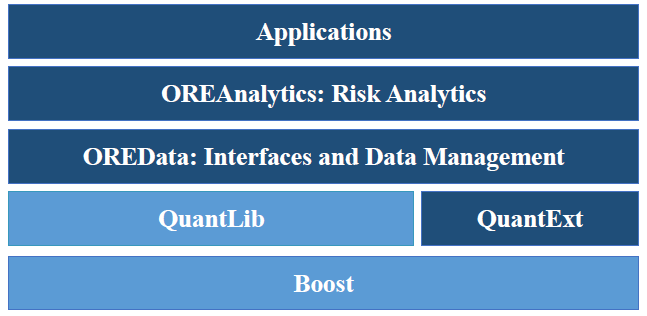
\includegraphics[scale=0.6]{data/Overview}
\end{center}
\caption{Hierarchy of ORE libraries. }
\label{fig_Hierarchy}
\end{figure}

The dark blue parts of indicate components of ORE, dependencies are indicated in light blue color.

\subsection*{QuantExt - Collection of QuantLib Extensions}

Extensions to QuantLib such as financial instruments, pricing models, pricing engines and term structures are collected in the QuantExt library. 
The internal organization of QuantExt (folder structure, class hierarchy) mimics the structure of QuantLib, so that developers familiar with QuantLib will have little difficulty finding their way around QuantExt as well.

At an early stage of the Open Source Risk project we decided to keep these kind of extensions separate from QuantLib (rather than adding to a local copy of the QuantLib library or immediately contributing these changes to the QuantLib project).
This facilitates QuantLib release changes, swapping QuantLib in ORE for another/newer version of QuantLib.

Similarly, rather than patching a copy of QuantLib locally when identifying a bug or issue, we tend to copy the affected QuantLib class or part of the QuantLib class hierarchy to QuantExt and apply the correction in QuantExt. In doing so, we decouple
from the QuantLib release cycle and bug fixes and facilitate quick fixes of parts of QuantLib that ORE critically depends on.

Some of the extensions that go into QuantExt may be contributed back into QuantLib with a delay, and then removed from QuantExt again. Examples are cross currency instruments and related engines and bootstrap helpers. Other extensions that are more
relevant for the risk analytics in ORE may stay in QuantExt longer term, such as the cross asset model underlying the Monte Carlo scenario generation for exposure simulation and xVA in ORE.

QuantLib's focus is on the individual instrument and its valuation and analysis whereas ORE aims at portfolio analytics that may be more than simply additive in the instrument's contributions (such as xVA, Value at Risk, etc). QuantExt provides
models and methods to support these analytics so that we might see QuantExt existing in parallel to QuantLib in the longer term.

\subsection*{OREData - Data Management, Translation and Assembly}

OREData is a library beyond the scope of QuantLib and QuantExt. OREData serves at the high level two purposes summarized under the label of ``data management''
\begin{itemize}
\item to {\bf translate} between external (XML) representations of financial objects and internal (C++) representations of objects in memory that QuantLib and QuantExt can deal with
\item to {\bf assemble essential object hierarchies} underneath the abstract
\begin{itemize}
\item {\bf Portfolio} object containing pointers to all financial products ``loaded''
\item {\bf Market} objects containing bootstrapped curves and volatility surfaces of all kinds) with the help of various kinds of {\bf configuration} and {\bf convention} objects
\item {\bf Model} objects used for market simulation or instrument pricing all with the help of a range of lower level {\bf utilities} and {\bf factories}. 
The functionality in OREData with QuantLib/QuantExt underneath is sufficient to build a market and bootstrap curves, load a portfolio from XML, calculate present values and project cash flows.
\end{itemize}
\end{itemize}

The key Portfolio, Market and Model objects are in turn used by the higher level analytics described in the next paragraph.

Furthermore, OREData provides supporting classes for reporting (see folder {\tt OREData/ored/report}) and various utility classes for building the above mentioned objects, logging, screen output and serialization (see folder {\tt OREData/ored/utility}).

\subsection*{OREAnalytics - Portfolio Risk Analytics}

OREAnalytics is a library that comprises the classes for portfolio risk analytics, in particular Monte Carlo simulation-based analytics. It was originally designed to support exposure simulation and XVA, but also covers hypothetical scenario analysis
(sensitivities, stress testing). The classes in OREAnalytics take the objects assembled in OREData (Portfolio, Market, Model) as an input. Key objects in OREAnalytics are then
\begin{itemize}
\item {\bf SimMarket} and derived classes, all derived in turn from the Market base class in OREData: allows changing market points and updates of term structures after market moves
\item {\bf ScenarioGenerator} classes of several kinds (LGM, cross asset model, sensitivity, stress test): these generate Monte Carlo or hypothetical market scenarios (stored in {\bf Scenario} objects);
the scenarios in turn can be ``applied'' to the ScenarioSimMarket, and a Portfolio linked to the latter market then reacts to the market changes when repriced
\item {\bf NPVCube}: interface to stored portfolio NPVs or sensitivities
\item {\bf ValuationEngine}: builds an NPV cube given Portfolio, SimMarket, simulation DateGrid; builds a sensitivity cube
\item {\bf PostProcess}: Performs NPV cube aggregation, evaluates the collateral account evolution, computes exposure statistics and XVAs; key inputs into PostProcess are the Portfolio, NettingSet data, today's market, the NPV cube generated by ValuationEngine
\item {\bf OREApp}: Orchestrates the information flow from portfolio and market data loading to various analytics and reporting, supports e.g. a batch type work flow for ORE as illustrated in figure \ref{fig_process}.
\end{itemize}

\begin{figure}[h]
\begin{center}
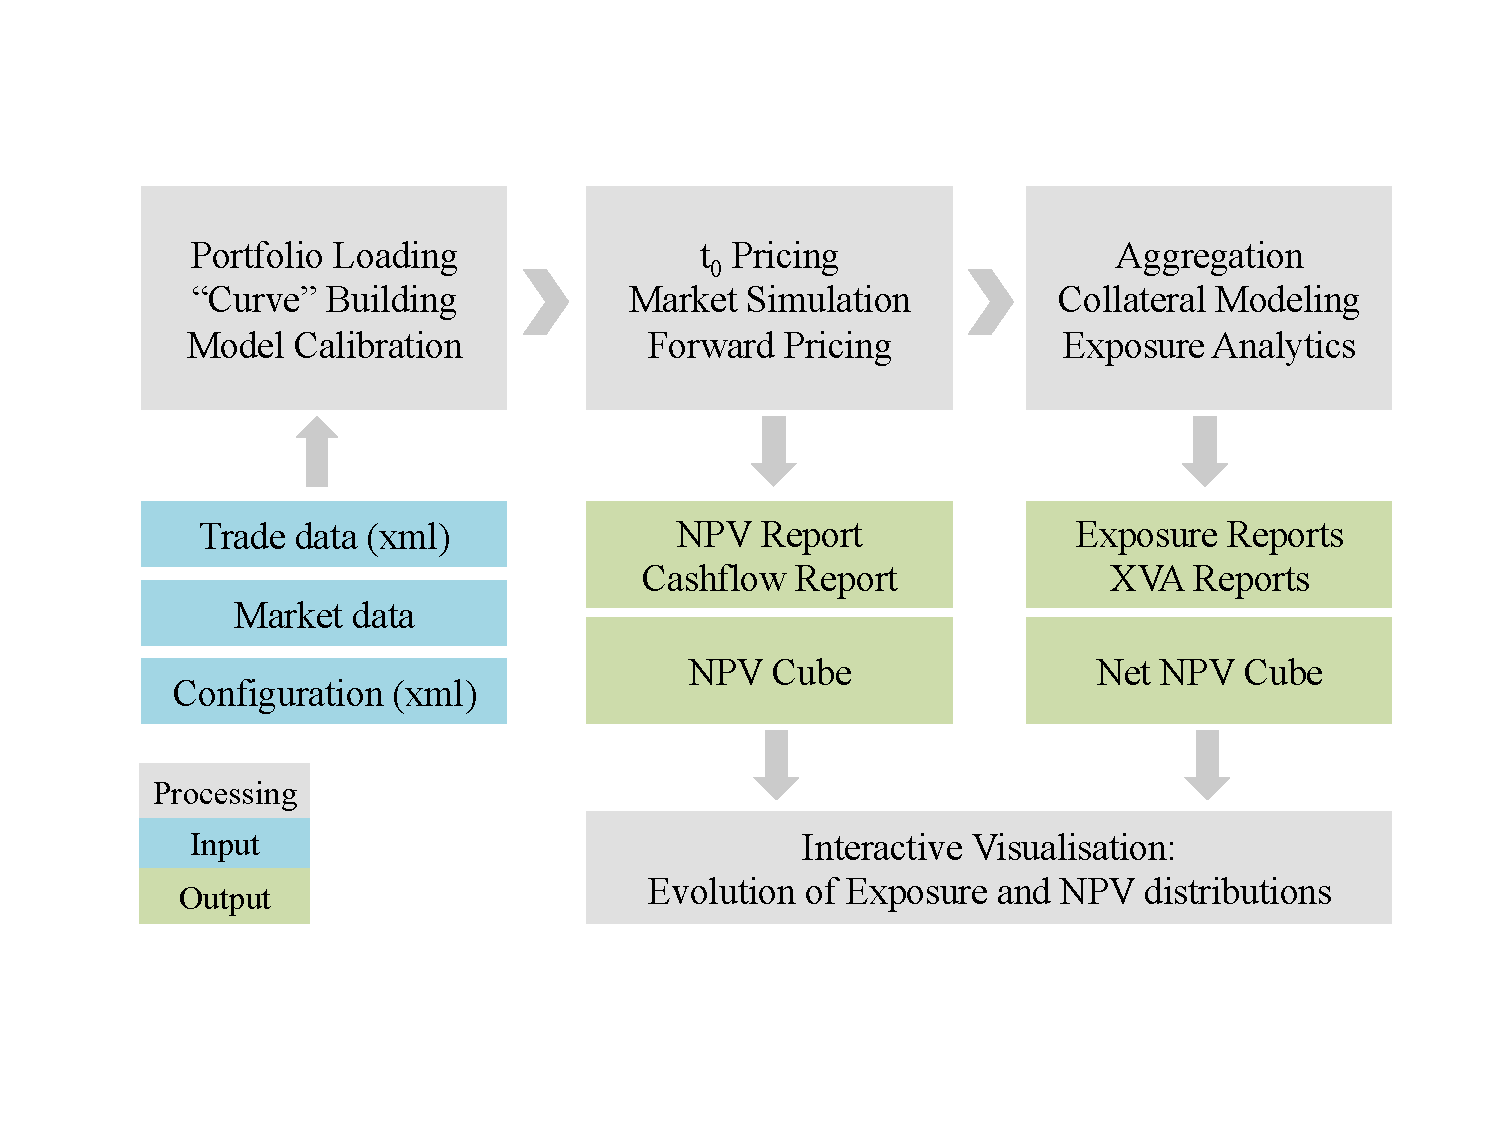
\includegraphics[scale=0.6]{data/process.pdf}
\end{center}
\caption{ Information flow implemented in ORE App. }
\label{fig_process}
\end{figure}


\subsection*{Applications}
ORE comes with a command line application that wraps the OREApp class in OREAnalytics, with the following minimal main function.

\begin{listing}[H]
%\hrule\medskip
\begin{minted}[fontsize=\footnotesize]{cpp}
int main(int argc, char** argv) {
	// ...
	if (argc != 2) {
		std::cout << endl << "usage: ORE path/to/ore.xml" << endl << endl;
		return -1;
	}
	string inputFile(argv[1]);
	boost::shared_ptr<Parameters> params = boost::make_shared<Parameters>();
	try {
		params->fromFile(inputFile);
		OREApp ore(params);
		return ore.run();
	} catch (const exception& e) {
		cout << endl << "an error occured: " << e.what() << endl;
		return -1;
	}
}
\end{minted}
\end{listing}

The ORE User Guide at \url{https://opensourcerisk.org/documentation} discusses the usage of the ORE command line application in detail, the main ore.xml input file passed to the application and the various inputs referenced therein.

\subsection*{Unit Tests}
All three libraries - QuantExt, OREData and OREAnalytics - are covered by unit test suites, again following the example of QuantLib. In total the test suites currently (as of release 11) comprise over 600 test cases.

\subsection*{Language Bindings}
To open ORE up and make its components accessible from other programming languages such as Python and Java, we pursue the same approach as QuantLib and provide (a framework of) language bindings using SWIG, the Simple Wrapper
Interface Generator (\url{http://swig.org}).

\begin{figure}[h]
\begin{center}
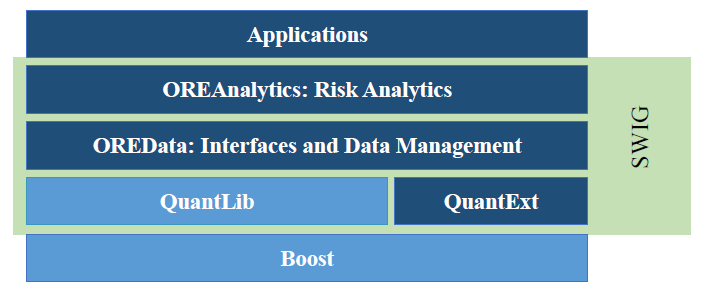
\includegraphics[scale=0.6]{data/OverviewSWIG}
\end{center}
\caption{SWIG wrapper. }
\label{fig_SWIG}
\end{figure}

The ORE SWIG bindings are open source as well and provided in a separate repository \url{https://github.com/opensourcerisk/ore-swig}). This project provides language bindings for QuantLib, QuantExt, OREData and OREAnalytics as illustrated in figure 
\ref{fig_SWIG}. This allows, for example, running the ORE process that is encapsulated in the C++ call {\tt ore.run()} in Python, but also querying members of the OREApp object in Python or calling into lower level OREData, QuantLib or QuantExt objects in Python. Refer to the examples in the ORE-SWIG project.

%------------------------------------------------------------------------------------------------------------
\section{Library Stack} 
%------------------------------------------------------------------------------------------------------------

\subsection{QuantExt}
QuantExt contains ORE's extensions to QuantLib such as financial instruments, pricing models, pricing engines and term structures, to extend the product coverage across six
asset classes ORE is aiming for. The internal organization of QuantExt (folder structure, class hierarchy) mimics the structure of QuantLib, so that developers familiar with QuantLib will have little difficulty finding their way around QuantExt as well.
Moreover we follow closely the design of QuantLib since
\begin{itemize}
\item QuantLib's design is based on decades of quant developer experience and well tested in practice over the past 20 years
\item we want to keep the option open that QuantExt code is migrated in part or entirely into QuantLib in the future
\end{itemize}

We do not elaborate on the QuantLib/QuantExt design and patterns, or the range of basic QuantLib objects here as this has been well covered by Luigi Ballabio, one of QuantLib's creators, in his reference book \cite{ballabio_book} with free drafts available in his blog posts \cite{ballabio_blog}.
In the following we sketch the current scope of the QuantLib extensions in QuantExt, as of the time of writing this text (Q1 2024). 
This concrete list is continuously changing and will be out of date at the time of the next release, i.e. check the on-line documentation at \url{https://www.opensourcerisk.org/docs/qle/index.html} for an up-to-date picture.

\begin{itemize}
\item {\bf Calendars}: Austria, Belgium, CME, Colombia, Cyprus, France, Greece, ICE, Ireland, Israel, Luxembourg, Malaysia, Mauritius, Netherlands, Peru, Philippines, Russia, Spain, Switzerland, UnitedArabEmirates; several additional calendars we added to QuantExt have been migrated into QuantLib by now; \\
  {\color{red}Note that ORE allows adding and amending calendars via configuration files and without code changes at the OREData level using amendedcalendar.xpp}
\item {\bf Cashflows} and related pricers for IR/FX/INF/EQ/COM payoffs:
  \begin{itemize}
  \item IR: Average overnight indexed coupon, Bond TRS cashflow, BRL CDI coupon, Capped/Floored Average BMA coupon, CMB coupon, Duration Adjusted CMS coupon, floating annuity coupon, IBOR FRA coupon, log-normal CMS spread pricer,, Overnight indexed coupon, scaled coupon, sub-period coupon
  \item IR/FX: FX linked notional coupon and cashflow, Fixed Rate FX linked notional coupon, Quanto coupon pricer
    \item INF: Non-standard capped/floored yoy inflation coupon, stripped capped/floored CPI coupon, stripped capped/floored YOY inflation coupon
  \item EQ: Equity coupon, Equity margin coupon
  \item Commodity: Commodity cashflow, commodity indexed average cashflow, Comodity indexed cashflow
  \end{itemize}
\item {\bf Currencies}: Various currencies added to QuantExt in the past have been migrated into QuantLib by now, four precious metal related currencies are left in QuantExt (XAU, XAG, XPT, XPD) \\
  {\color{red}Note that currencies can be added now via configuration and without code changes at the OREData level using configurablecurrency.xpp}
% Africa (TND, EGP, NGN, MAD), America (MXV, CLF), Asia (KZT, QAR, BHD, OMR, AED, PHP, CNH), Precious Metals
\item {\bf Indexes}: Inflation indices (BE HI CP, CA CPI, DE CPI, DK CPI, ES CPI, FR CPI SE CPI)Bond index, Commodity index, Commodity basis future index, Equity index, Compo Equity index, FX index, Inflation indices (CA CPI, Danish CPI, Swedish CPI), and a range of 48 IBOR indices connected with the additional currencies above;\\
 {\color{red}Note that additional overnight and IBOR indices can be created in ORE via conventions, i.e. without code changes in QuantExt or QuantLib}
\item {\bf Instruments}: About 50 instruments across asset classes
  \begin{itemize}
    \item IR: Average OIS, BRL CDI Swap, Cash-settled European Option, Deposit, Double Overnight Indexed Basis Swap, Fixed BMA Swap, Credit-linked Swap, Multi Currency Composite instrument, Multi-Leg Option, OIS Basis Swap, Sub Periods Swap,  Tenor Basis Swap
    \item IR/FX: FX Forward, Cross Currency Basis MTM Reset Swap, Cross Currency Basis Swap, Cross Currency Fixed/Float Swap, Cross Currency Swap, Currency Swap, Overnight Indexed Cross Currency Basis Swap
    \item Equity/FX: Cliquet Option, Variance Swap, Equity Forward, Variance Swap, Vanilla Forward Option
  \item Commodity: Commodity Average Price Option, Commodity Forward, Commodity Spread Option
  \item Credit: Collateralized Bond Obligation, CDS Option, Credit Default Swap, Risk Participation Agreement, Synthetic CDO,
    \item Bond: Bond Option, Bond Repo, Bond Total Return Swap, Convertible Bond, ASCOT, Forward Bond, Implied Bond Spread Helper
   \end{itemize}
  {\color{red}Note that the scripted trade framework, which allows defining further instruments via payoff scripts, currently resides in OREData, see below}
\item {\bf Math}: Various tools used in models and engines
  \begin{itemize}
  \item Risk: Delta Gamma VaR, bucketed distribution, kendall rank correlation, covariance salvage
    \item Par sensitivity conversion: block matrix inverse
    \item Interpolation/Extrapolation: constant interpolation, quadratic interpolation, logquadratic interpolation, flat extrapolation
    \item Regression: Nadaraya Watson Regression, Stabilized General Linear Least Squares Fit
    \item Optimisation: Multi-threaded differential evolution
    \item Classes used in the scripted framework: Basic CPU environment, compute environemnt, opencl environment, compiled formula, random variable operations, random variable LSM basis system
  \end{itemize}
\item {\bf Methods}:
  \begin{itemize}
  \item Monte Carlo: Brownian Bridge Path interpolator, multi-path generator, multi path variate generator, path generator factory,  projected buffered multi-path generator and factory
  \item Finite Difference: Black Scholes mesher, Black Scholes operator, defaultable equity jump diffusion Fokker Planck operator, Quanto helper
  \end{itemize}
\item {\bf Models} used for pricing and market simulation for Exposure and xVA: 
  \begin{itemize}
  \item Model and model parameterization classes: Linear Gauss Markov Model (LGM), Cross Asset Model, Cross Asset Analytics, Cross Asset Model Parametrization (EQ BS Constant / Piecewise Constant, FX BS Constant/ Piecewise Constant, IR LGM1F Constant / Piecewise Linear / Constant HullWhite, INF DK, CR LGM1F), Projected Cross Asset Model, Gaussian 1d Cross Asset adaptor, Multi-Factor Hull-White model, Normal SABR and Normal SABR interpolation, Linkable Calibrated model, Defaultable Equity Jump Diffusion model, LGM Vectorised
  \item Model calibration helpers: CMS Cap, CPI Cap/Floor, CDS Option, FX/EQ Option, Futures Option, representaive swaption and fxoption
  \item Model Implied Termstructures: DK Zero Inflation, DK YOY Inflation, LGM Credit, LGM Yield, CIR++ Default, exact Bachelier implied volatility, implied price/yield term structure,
  \item Basket credit models and methods: homogeneous pool, pool loss model, Gaussian Large Homogeneous Pool loss model, Hull White bucketing, transition matrix)
  \item Carr-Madan arbitrage check
    \end{itemize}
\item {\bf Pricing Engines}: About 60 pricing engines covering the additional instruments and models above
  \begin{itemize}
  \item IR: Analytic LGM Swaption, Deposit, Swap Delta, Swap Multi Curve, LGM Convolution Solver, Numeric LGM Swaption, Deposit, LGM Convolution Solver, Monte Carlo AMC LGM Swap, MC AMC LGM Swaption, MC AMC Multi-Leg Option, Numeric LGM Multi-Leg Option
  \item IR/FX: Analytic Cross Currency LGM FX Option, Barone Adesi Whaley, Cross Currency Swap, Currency Swap, FX Forward, Monte Carlo AMC Currency Swap, MC AMC FX Forward, MC AMC FX Option, Overnight Index Cross Currency Basis Swap
  \item INF: Analytic DK CPI Cap/Floor, CPI Bachelier Cap/Floor, CPI Black Cap/Floor, Analytic JY CPI Cap/Floor, Analytic JY YoY Cap/Floor 
  \item Equity/FX: Analytic Cross Asset LGM Equity Option, Equity Forward, FX Forward, Overnight Index Cross Currency Basis Swap, Analytic Barrier Option, Analytic Cash-Settled European Swaption,  Analytic LGM FX Option, Analytic Digital American Option, Analytic Double Barrier Binary Option, Analytic Double Barrier Option, Analytic European Option, Analytic European Forward Option, Analytic Cross Asset LGM Equity Option, Barone Adesi Whaley, Equity Forward, Variance Swap General Replication, Volatility From Variance Swap
  \item Commodity: Commodity Forward, Commodity APO, Commodity Schwartz Future Option, Commodity Spread Option, Commodity Swaption, Discounting Commodity Forward
  \item Credit: Analytic LGM CDS Option, Black CDS Option, Black Index CDS Option, Midpoint CDS, Midpoint CDS Mutli-State, Midpoint Index CDS, Numerical Integration Index CDS Option, Analytic LGM CDS Option, Credit-Linked Swap, Index Tranche, Midpoint CDO, idpoint
  \item Bond: Risky Bond, Accrual Bond Repo, Binomial Convertible, Black Bond Option, CBOMonte Carlo, Bond Repo, Bond TRS, Forward Bond, Risky Bond, Risky Bond Multi-State, Finite Difference Convertible Bond, Finite Difference Defaultable Equity Jump Diffusion, Intrinsic Ascot
  \end{itemize}  
\item {\bf Processes}: Cross Asset State Process, IR LGM1F State Process, IR HW State Process, CIR++ State Process, Commodity Schwartz State Process
\item {\bf Quotes}: Log Quote, Base Correlation Quote, Composite Vector Quote
\item {\bf Term Structures}: About 80 term structures and helper classes supporting the pricing across six asset classes
\begin{itemize}
\item {\bf Bootstrap Helpers}: Average OIS Rate Helper, Basis Two Swap Helper, BRL CDI Rate Helper, Cap/Floor Helper, Cross Currency Basis MTM Reset Swap Helper, Cross Currency Basis Swap Helper, Cross Currency Fix/Float Swap Helper, IMM FRA Rate Helper, Dated Stripped Optionlet and Adapter, Default Probability Helpers, Equity Forward Curve Stripper, Overnight Index Basis Swap / Cross Currency Basis Swap, Sub-Periods Swap, Tenor Basis Swap
\item {\bf Black Volatility Term Structures}: Inverted Vol, Monotone Variance, Variance Moneyness, Surface with Delta, Surface with ATM, Sparse Surface, 
\item {\bf Dynamic Termstructures}: Black Vol Termstructure, Optionlet Vol Termstructure, Swaption Vol Matrix, YOY Optionlet Vol Termstructure
\item {\bf Spreaded Termstructures}: Spreaded Optionlet Volatility, Spreaded Smile Section, Spreaded Swaption Volatility, Equity Vol Constant Spread, Hazard Spreaded Default Termstructure
\item {\bf FX}: Black Vol Surface, Smile Section, Vanna Volga Smile Section
\item {\bf Inflation}: Stripped CPI Volatility Structure, Stripped YOY Inflation Optionlet Volatility, YOY Inflation Optionlet Stripper, YOY Optionlet Volatility Surface, corrections of QuantLib's ``KInterpolatedYoYOptionletVolatilitySurface''
\item {\bf Correlation}: Correlation Termstructure, Flat Correlation Termstructure
\item {\bf Others}: Cap/Floor Term Vol Curve, Cap/Floor Term Vol Surface, Cross Currency Price Termstructure, Discount Ratio Modified Curves, Price Term Structure and Adapter, Extension of QuantLib's Iterative Bootstrap, corrections and extensions to QuantLib's Optionlet Stripper
\end{itemize}
\item {\bf Time}: Year Counter, Futures Expiry Calculator
\end{itemize}

The current size of the QuantExt code base is about 125k source lines (excluding blank lines). ORE's size across the three libraries in ORE is 350k lines. QuantLib's size is about 476k lines.

\subsection{ORE Data}
The Data management library OREData, as stated above, hosts the classes for
\begin{itemize}
\item translating external trade, market and configuration data into financial objects that QuantExt and QuantLib can deal with, and
\item assembling these into object hierarchies the higher level analytics can use  conveniently (e.g. Portfolio, Market, Pricing Models, Simulation Models)
\end{itemize}

The OREData library currently comprises about 149 thousand lines of code and exceeds the size of QuantExt.

We start illustrating OREData's design by focusing on the Market objects.

\subsubsection{Market Data}\label{sec:marketdata}
The market base class provides the interface to all kinds of term structure objects that might be needed in pricing across asset classes. Listing \ref{1st:marketdata} shows a small excerpt, all member functions are pure virtual and are implemented in derived classes. It is then
sufficient to pass a smart pointer respectively Handle to a base Market object into classes or functions that need to perform pricing. Relevant term structures, indices and quotes are queried by providing a single unique key or set of keys.

The Market interface covers
\begin{itemize}
\item Yield term structures by type and name, as shown in listing \ref{1st:marketdata}
\item Swaption volatility structures by currency
\item Discount curves by currency
\item IBOR and Swap indices (with associated forward curves) by index name
\item FX Spot quotes by currency pair
\item FX volatility term structures by currency pair
\item Default term structures by name
\item Recovery rate quotes by name
\item CDS volatility term structures by name
\item Base correlation term structures by qualifier
\item Zero and Year-on-Year inflation indices (with associated forward curves) by index name
\item Cap/Floor volatility structures by currency
\item Year on year Cap/Floor volatility and price surfaces by index name
\item Zero inflation Cap/Floor volatility and price surfaces by index name
\item Equity spot prices, dividend and forecasting curves by equity name
\item Equity volatility term structures by equity name
\item Security spreads by security ID
\item Commodity price curves by commodity name
\item Commodity volatility term structures by commodity name
\item Generic correlation term structures by index pair
\item Prepayment rate quotes by security ID
\end{itemize}

\begin{listing}[H]
%\hrule\medskip
\begin{minted}[fontsize=\footnotesize]{cpp}
class Market {
public:
virtual ~Market() {}
virtual Date asofDate() const = 0;
//! \name Yield Curves
//@{
virtual Handle<YieldTermStructure>
discountCurve(const string& ccy,
const string& configuration = Market::defaultConfiguration) const = 0;
virtual Handle<IborIndex>
iborIndex(const string& indexName,
const string& configuration = Market::defaultConfiguration) const = 0;
virtual Handle<SwapIndex>
swapIndex(const string& indexName,
const string& configuration = Market::defaultConfiguration) const = 0;
//@}
//! \name Swaptions
//@{
virtual Handle<SwaptionVolatilityStructure>
swaptionVol(const string& ccy,
const string& configuration = Market::defaultConfiguration) const = 0;
// ...
//@}
//! \name Foreign Exchange
// ...
};
\end{minted}
\caption{Market base class, pure virtual member functions with varying number and type of keys and common last argument indicating the ``curve ID'' to select one of several market configurations.}
\label{1st:marketdata}
\end{listing}

The {\tt MarketImpl} class is derived from {\tt Market}, and it essentially provides member variables (maps) to store the underlying term structures, indices and quotes.
The {\tt TodaysMarket} class is derived from {\tt MarketImpl}, and it provides a constructor that builds a concrete Market instance. 
This build process involves various helper classes for each term structure across the asset classes, see folder {\tt OREData/ored/marketdata}, as well as configuration helpers for each term structure in folder {\tt OREData/ored/configuration}. Moreover, the build process involves
\begin{itemize}
\item reading market data in csv files and term structure configurations data XML files into internal data classes, and
\item parsing/translating text into basic QuantLib/QuantExt objects such as Calendars, Periods, Currencies, Quotes etc., all supported by the utility code assembled in folder {\tt OREData/ored/utilities}.
\end{itemize}
The {\tt TodaysMarket} class is sufficient for portfolio pricing. Further derived classes that are essential for market simulation and scenario analysis are introduced in the next section on OREAnalytics.

\subsubsection{Portfolio and CSA Data}

\begin{listing}[H]
%\hrule\medskip
\begin{minted}[fontsize=\footnotesize]{cpp}
class Portfolio {
public:
//! Get a Trade with the given trade id from the portfolio
boost::shared_ptr<Trade> get(const std::string& id) const;
//! Load using a default or user supplied TradeFactory
void load(const std::string& fileName,
const boost::shared_ptr<TradeFactory>& tf = boost::make_shared<TradeFactory>());
//! Load from an XML string using a default or user supplied TradeFactory
void loadFromXMLString(const std::string& xmlString,
const boost::shared_ptr<TradeFactory>& tf
= boost::make_shared<TradeFactory>());
//! Load from XML Node
void fromXML(XMLNode* node,
const boost::shared_ptr<TradeFactory>& tf
= boost::make_shared<TradeFactory>());
//! Save portfolio to an XML file
void save(const std::string& fileName) const;
//! Call build on all trades in the portfolio
void build(const boost::shared_ptr<EngineFactory>&);
//! Return trade list
const std::vector<boost::shared_ptr<Trade>>& trades() const { return trades_; }
// ...
};
\end{minted}
\caption{Excerpt of the Portfolio class showing essential member functions.}
\label{1st:portfolio}
\end{listing}

The second large part of OREData deals with trade loading and building from external sources and assembling all trades in a {\tt Portfolio} object. An excerpt is shown in listing \ref{1st:portfolio}. The {\tt Portfolio} class provides several ways of loading a portfolio (from an
XML file, an XML string, a single XML node), to store a portfolio to XML file, to access individual trades. When a portfolio is loaded from an external source, it is first represented in internal trade objects where all relevant fields are native (string, integer, double, bool) variables
or standard C++ containers like vectors or maps.

In a subsequent step, initiated by a call to the {\tt build} member function, the ``raw'' trade data is then translated into QuantLib/QuantExt objects up to the QuantLib/QuantExt instrument, linked to a QuantLib/QuantExt pricing engine, in turn linked to the relevant term structures provided by the {\tt Market} class introduced in Section \ref{sec:marketdata}.
The role of the {\tt TradeFactory} class in the Portfolio member functions is to help constructing concrete instances of trade objects depending on the TradeType information in the trade XML representation.
All trade objects derive from a common {\tt Trade} base class shown in listing \ref{1st:trade}.

\begin{listing}[H]
%\hrule\medskip
\begin{minted}[fontsize=\footnotesize]{cpp}
class Trade {
public:
class Trade : public XMLSerializable {
public:
// Constructor
// ....
//! Build QuantLib/QuantExt instrument, link pricing engine
virtual void build(const boost::shared_ptr<EngineFactory>&) = 0;
//! Return fixings that are relevant for pricing
virtual std::map<std::string, std::set<QuantLib::Date>>
fixings(const QuantLib::Date& settlementDate = QuantLib::Date()) const = 0;
//! \name Serialisation
//@{
virtual void fromXML(XMLNode* node);
virtual XMLNode* toXML(XMLDocument& doc);
//@}
//! \name Inspectors
//@{
const string& id() const { return id_; }
const string& tradeType() const { return tradeType_; }
const Envelope& envelope() const { return envelope_; }
const set<string>& portfolioIds() const { return envelope().portfolioIds(); }
const TradeActions& tradeActions() const { return tradeActions_; }
const boost::shared_ptr<InstrumentWrapper>& instrument() { return instrument_; }
const std::vector<QuantLib::Leg>& legs() { return legs_; }
const std::vector<string>& legCurrencies() { return legCurrencies_; }
const std::vector<bool>& legPayers() { return legPayers_; }
const string& npvCurrency() { return npvCurrency_; }
const Date& maturity() { return maturity_; }
//@}
//...
};
\end{minted}
\caption{Excerpt of the Trade class showing essential member functions.}
\label{1st:trade}
\end{listing}

The {\tt Trade} class provides access to the underlying QuantLib/QuantExt instrument and further trade information that is meaningful across all kinds of products. There is a range of concrete classes derived from {\tt Trade} that perform the actual load and build process, see folder {\tt OREData/ored/portfolio}. The list of ORE trade types up to release 6 in July 2021 was
\begin{itemize}
\item Bond
\item Cap/Floor
\item Commodity Forward, European Commodity Option
\item Credit Default Swap
\item Equity Forward, Equity Swap, European Equity Option
\item Forward Bond
\item Forward Rate Agreement
\item FX Forward, FX Swap, European and American FX Option
\item Swap
\item European and Bermudan Swaption
\end{itemize}

The product coverage has then grown significantly to about 100 types over five quaterly releases, with Quaternion/Acadia contributing the bulk of formerly proprietary code to ORE. As of release 11:
\begin{itemize}
      \item CompositeTrade
      \item ConvertibleBond
      \item Ascot
      \item TotalReturnSwap
      \item ContractForDifference
      \item CBO
      \item EquityPosition
      \item EquityOptionPosition
      \item BondPosition
      \item MultiLegOption
      \item IndexCreditDefaultSwap
      \item IndexCreditDefaultSwapOption
      \item SyntheticCDO
      \item BondOption
      \item BondTRS
      \item BondRepo
      \item CreditLinkedSwap
      \item CrossCurrencySwap
      \item InflationSwap
      \item Swap
      \item Swaption
      \item ForwardRateAgreement
      \item FxAverageForward
      \item FxForward
      \item FxOption
      \item FxAsianOption
      \item FxBarrierOption
      \item FxDoubleBarrierOption
      \item FxSwap
      \item FxDigitalOption
      \item FxEuropeanBarrierOption
      \item FxKIKOBarrierOption
      \item FxTouchOption
      \item FxDoubleTouchOption
      \item FxDigitalBarrierOption
      \item FxVarianceSwap
      \item CapFloor
      \item EquityOption
      \item EquityFutureOption
      \item EquityAsianOption
      \item EquityBarrierOption
      \item EquityDoubleBarrierOption
      \item EquityEuropeanBarrierOption
      \item EquityTouchOption
      \item EquityDoubleTouchOption
      \item EquityDigitalOption
      \item EquityForward
      \item EquitySwap
      \item EquityVarianceSwap
      \item EquityCliquetOption
      \item CommodityForward
      \item CommodityOption
      \item CommodityDigitalAveragePriceOption
      \item CommodityDigitalOption
      \item CommodityAsianOption
      \item CommoditySwap
      \item CommoditySwaption
      \item CommoditySpreadOption
      \item CommodityAveragePriceOption
      \item CommodityOptionStrip
      \item CommodityPosition
      \item CommodityVarianceSwap
      \item Bond
      \item ForwardBond
      \item CreditDefaultSwap
      \item CreditDefaultSwapOption
      \item Failed
      \item ScriptedTrade
      \item EquityBasketVarianceSwap
      \item FxBasketVarianceSwap
      \item CommodityBasketVarianceSwap
      \item RiskParticipationAgreement
      \item Autocallable\_01
      \item DoubleDigitalOption
      \item EuropeanOptionBarrier
      \item PerformanceOption\_01
      \item FxTaRF
      \item EquityTaRF
      \item CommodityTaRF
      \item FxWorstOfBasketSwap
      \item EquityWorstOfBasketSwap
      \item CommodityWorstOfBasketSwap
      \item EquityBestEntryOption
      \item FxBestEntryOption
      \item CommodityBestEntryOption
      \item FxAccumulator
      \item EquityAccumulator
      \item CommodityAccumulator
      \item FxWindowBarrierOption
      \item EquityWindowBarrierOption
      \item CommodityWindowBarrierOption
      \item FxGenericBarrierOption
      \item EquityGenericBarrierOption
      \item CommodityGenericBarrierOption
      \item FxBasketOption
      \item EquityBasketOption
      \item CommodityBasketOption
      \item FxRainbowOption
      \item EquityRainbowOption
      \item CommodityRainbowOption
      \item KnockOutSwap
 \end{itemize}

The trade design is modular, and objects re-used within various trade types as member variables are
\begin{itemize}
\item Envelope
\item Schedule
\item OptionData
\item LegData
\item TradeActions
\end{itemize}
each of which comes with functions for loading from XML, building QuantLib/QuantExt objects.

{\bf CSA Data} is represented in a single class, {\tt NettingSetDefinition}, see folder {\tt OREData/ored/portfolio}, also XML serializable like each trade. The ``portfolio'' of CSAs is then managed by class {\tt NettingSetManager}, 
XML serializable like the {\tt Portfolio} object.

\subsubsection{Pricing Engines, Engine Factory}
Each trade is linked with a pricing engine during the trade's build process. In order to limit the number of engines to be constructed (and to limit memory usage), ORE reuses engines as far as possible. This is achieved by the {\tt EngineBuilder},
{\tt EngineFactory} and {\tt LegBuilder} classes. Currently, ORE provides 36 concrete ``default'' engine and leg builders when the {\tt EngineFactory} is constructed, see orea/app/initbuilders.cpp. The design here is extensible so that developers can add their own engine builders to the
factory when extending ORE. For this purpose the {\tt EngineFactory} class provides the {\tt addExtraBuilders} member function.

Figure \ref{fig_OREDPortfolio} shows the relationships of these classes:

\begin{figure}[h]
\begin{center}
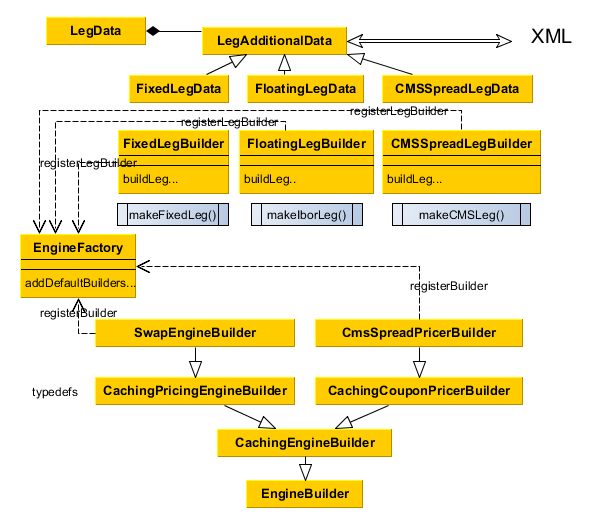
\includegraphics[scale=0.6]{data/ORED_Portfolio}
\end{center}
\caption{Collaboration Diagram of Instrument/Leg Builder and Factory Classes}
\label{fig_OREDPortfolio}
\end{figure}

\subsubsection{Pricing Models and Simulation Models}
The construction and calibration of Pricing and Simulation models is encapsulated in the {\tt LgmBuilder} and {\tt CrossAssetModelBuilder} classes, see folder {\tt OREData/ored/models}. Both are supported by associated ``data'' classes that hold
the model/calibration configuration, XML serializable like portfolio and other configuration data in ORE.

\subsubsection{Scripting}

With the 11th release we added the scripted trade instrument which allows representing a variety of payoffs (cross asset classes, path-dependent, with multiple early exercise features) using a scripting language. The bulk of the related code can be found in OREData/ored/scripting and supports the construction and processing of the scripted trade instrument that is build in OREData/ored/portfolio/scriptedtrade.cpp. We drill deeper into the design of the scripted trade and its processing in Section \ref{sec:scriptedtrade}.

\subsection{ORE Analytics}

The OREAnalytics library comprises the classes for portfolio risk analytics, in particular Monte Carlo simulation-based analytics. It was originally designed to support exposure simulation and XVA, but also covers hypothetical scenario analysis
(sensitivities, stress testing). The classes in OREAnalytics depend on QuantLib, QuantExt and OREData, and the primary inputs into analytics are the Portfolio, Market and CrossAssetModel objects introduced in section \ref{sec:marketdata}.

The OREAnalytics library currently comprises about 80 thousand lines of code, somewhat smaller than QuantExt and OREData.

\subsubsection{Simulation Market}
The {\tt TodaysMarket} class in OREData provides a snapshot of the market as of a given reference date. The Portfolio is linked to this market to produce the reference date's valuations and cash flow projections. ORE's design to support analysis of how
valuations change when the market moves under hypothetical scenarios with fixed reference date or under market changes through time is to ``simply'' link the portfolio to a market that change in these ways and then triggers repricing. 
The key element for the implementation is the {\tt SimMarket} class, derived from the {\tt MarketImpl} (which is derived form {\tt Market}), i.e. it provides the same interfaces, and some additional and essential member functions, 
in particular the {\tt update} function, as shown in listing \ref{1st:simmarket}, see folder {\tt OREAnalytics/orea/simulation}.

\begin{listing}[H]
%\hrule\medskip
\begin{minted}[fontsize=\scriptsize]{cpp}
class SimMarket : public data::MarketImpl {
public:
SimMarket(const Conventions& conventions) : MarketImpl(conventions), numeraire_(1.0) {}
//! Generate or retrieve market scenario, update market, notify termstructures and update fixings
virtual void update(const Date&) = 0;
//! Return current numeraire value
Real numeraire() { return numeraire_; }
//! Reset sim market to initial state
virtual void reset() = 0;
//! Get the fixing manager
virtual const boost::shared_ptr<FixingManager>& fixingManager() const = 0;
protected:
Real numeraire_;
};
\end{minted}
\caption{Simulation Market base class.}
\label{1st:simmarket}
\end{listing}

The concrete class that derives from {\tt SimMarket} and that actually implements {\tt update}, {\tt reset} and {\tt fixingManager} is {\tt ScenarioSimMarket}, as shown in listing \ref{1st:scenariosimmarket}, see folder {\tt OREAnalytics/orea/scenario}.

\begin{listing}[H]
%\hrule\medskip
\begin{minted}[fontsize=\scriptsize]{cpp}
//! Simulation Market updated with discrete scenarios
class ScenarioSimMarket : public analytics::SimMarket {
public:
//! Constructors
// ...
//! Set scenario generator
boost::shared_ptr<ScenarioGenerator>& scenarioGenerator() { return scenarioGenerator_; }
//! Set aggregation data
boost::shared_ptr<AggregationScenarioData>& aggregationScenarioData() { return asd_; }
//! Set scenarioFilter
boost::shared_ptr<ScenarioFilter>& filter() { return filter_; }
//! Update market snapshot and relevant fixing history
void update(const Date& d) override;
//! Reset sim market to initial state
virtual void reset() override;
//! Return the fixing manager
const boost::shared_ptr<FixingManager>& fixingManager() const override { return fixingManager_; }
// ...
};
\end{minted}
\caption{Excerpt of the concrete Simulation Market class.}
\label{1st:scenariosimmarket}
\end{listing}

The {\tt ScenarioGenerator} class that appears here is used to generate single or multiple market scenarios. This is used in ScenarioSimMarket's {\tt update} function which then
applies the generated scenario to the underlying data in {\tt ScenarioSimMarket}. Moreover, the update call triggers QuantLib observer notification chains so that the portfolio that is linked to {\tt ScenarioSimMarket} reacts to these changes with amended
valuations when asked for NPVs next time. To finish this section we note that the configuration for the simulation market's composition is externally done in ORE XML, and there is a configuration class {\tt ScenarioSimMarketParameters} which is XML (de-)serializable, and used in the construction of the {\tt ScenarioSimMarket} object.

\subsubsection{Scenario Generation}
OREAnalytics covers two types of Monte Carlo scenario generators that produce market evolutions - {\tt LgmScenarioGenerator} for risk neutral interest rate scenarios only,
{\tt CrossAssetModelScenarioGenerator} for IR/FX/INF/EQ market scenarios, as well as sensitivity and stress testing scenario generators {\tt SensitivityScenarioGenerator} and {\tt stressScenarioGenerator}. 
All generators have associated XML (de-)serializable configuration classes which are used to construct the generators. 
The interface between any scenario generator and the {\tt ScenarioSimMarket} is the {\tt Scenario} object shown in listing \ref{1st:scenario}. Its concrete derived classes hold the actual generated data.

\begin{listing}[H]
%\hrule\medskip
\begin{minted}[fontsize=\scriptsize]{cpp}
class Scenario {
public:
//! Return the scenario asof date
virtual const Date& asof() const = 0;
//! Get the scenario label
virtual const string& label() const = 0;
//! Set the scenario label
virtual void label(const string&) = 0;
//! Get Numeraire ratio n = N(t) / N(0) so that Price(0) = N(0) * E [Price(t) / N(t) ]
virtual Real getNumeraire() const = 0;
//! Set the Numeraire ratio n = N(t) / N(0) so that Price(0) = N(0) * E [Price(t) / N(t) ]
virtual void setNumeraire(Real n) = 0;
//! Check whether this scenario provides the data for the given key
virtual bool has(const RiskFactorKey& key) const = 0;
//! Risk factor keys for which this scenario provides data
virtual const std::vector<RiskFactorKey>& keys() const = 0;
//! Add an element to the scenario
virtual void add(const RiskFactorKey& key, Real value) = 0;
//! Get an element from the scenario
virtual Real get(const RiskFactorKey& key) const = 0;
//! clones a scenario and returns a pointer to the new object
virtual boost::shared_ptr<Scenario> clone() const = 0;
// ...
};
\end{minted}
\caption{Excerpt of the Scenario data class.}
\label{1st:scenario}
\end{listing}

The scenario object refers to a unique reference date and contains an arbitrarily large number of data points that are identified by a RiskFactorKey. The key identifies the risk factor class (25 types so far in ORE, see the definition in
{\tt OREAnalytics/orea/scenario/scenario.hpp}, e.g. {\tt DiscoutCurve}, {\tt IndexCurve}, {\tt SwaptionVolatility}, etc.), a name (e.g. a currency or index name), and an integer indicating the position of the data item in a vector, matrix or cube. A market
evolution or path is hence represented by a vector of scenarios. So far there is only one derived class from the base Scenario in ORE, {\tt SimpleScenario}, which stores the scenario data in simple vectors and maps, also serializable.

\subsubsection{Engine}
The {\tt OREAnalytics/orea/engine} folder comprises a number of calculators (wrapped into individual classes) for ORE's risk analytics beyond single pricing as of the reference date:
\begin{itemize}
\item {\bf ValuationEngine} - performs a market simulation, prices a portfolio under scenarios, possibly through time, and fills a resulting NPV cube, with the help of the ValuationCalculator class; the ValuationEngine is used for Monte Carlo simulations of the market evolution but also the hypothetical scenario analytics below
\item {\bf SensitivityAnalysis}, also performed with the help of ValuationEngine and ValuationCalculator: This class wraps functionality to perform a sensitivity analysis for a given portfolio.
\begin{itemize}
\item builds the "simulation" market to which sensitivity scenarios are applied, 
\item builds the portfolio linked to this simulation market
\item generates sensitivity scenarios
\item runs the scenario "engine" to apply these and compute the NPV impacts of all required shifts
\item compiles first and second order sensitivities for all factors and all trades
\item fills result structures that can be queried
\end{itemize}
\item {\bf StressTest}, also performed with the help of ValuationEngine and ValuationCalculator: This class wraps functionality to perform a stress testing analysis for a given portfolio and
\begin{itemize}
\item builds the "simulation" market to which stress scenarios are applied, 
\item builds the portfolio linked to this simulation market
\item generates stress scenarios
\item runs the scenario "engine" to apply these and compute the NPV impacts of all required shifts
\item fills result structures that can be queried
\item writes stress test report to a file
\end{itemize}
\item {\bf ParametricVarCalculator}, as post-processor of a SensitivityStream, takes sensitivity data
  and a covariance matrix as an input and computes a parametric value at risk. The output can be
  broken down by portfolios, risk classes (IR, FX, EQ, ...) and risk types (delta-gamma, vega, ...)
\item {\bf CounterpartyCalculator/SurvivalProbabilityCalculator}, calculates the survival probability
  of a counterpart to be stored in the resulting cube
\item {\bf ParSensitivityAnalysis} \\ 
  The sensitivity analysis class above computes sensitivities to changes in zero rates, hazard rates,
  optionlet volatilities, inflation zero rates. The ParSensitivityAnalysis class turns these ``raw''
  sensitivities into ``par'' sensitivities (i.e. sensitivities to changes in Deposit rates, Swap
  rates, CDS spreads etc.) via Jacobi transformation i.e. using the chain rule of differentiation.
  The Jacobi matrix for this purpose is given by the sensitivity of par instruments to the underlying
  ``raw domain'' risk factors, and it is computed in ORE by bump \& revalue.
  This yields a possibly very large sparse Jacobi matrix. Transforming the portfolio's
  raw sensitivities into par sensitivities involves multiplying the portfolio's raw sensitivity vector
  with the {\em inverse} of the Jacobi matrix. While conceptually simple, the implementation is
  involved and fills 2500+ lines of code in a single class.  Sensitivity analysis in the raw domain is
  faster than direct sensitivity analysis in the par domain, because it avoids repeated curve
  bootstraps after changing market points that feed into curves.
\item {\bf MultithreadedValuationEngine} \\
  Quoting Luigi Ballabio: ``{\em QuantLib is generally not
  thread-safe. The thread-local singleton pattern gives you per-thread singletons instead of global
  ones, but it doesn't prevent race conditions if you share objects between threads... I suggest to
  use multiple processes instead.}'' In ORE we have chosen a middle way to parallise processing using
  ``isolated'', process-like, threads as follows: The engine builds the full portfolio once and
  prices it in the ``main thread''.
  Then it splits the portfolio into N parts with similar pricing time and spawns
  N threads. Within each thread, the engine sets the essential thread-local singleton
  (the evaluation date), builds a clone of the full market, builds a local scenario sim market, builds
  the respective sub-portfolio linked to the thread's local market, builds and runs the usual
  ValuationEngine; the engine then populates a ``mini netting set NPV cube'' for
  the sub-portfolio. Because the engine parallelises by splitting the portfolio and because market
  building causes a fixed computational overhead, we need a sufficiently large full portfolio and
  sufficiently large sub-portfolios to achieve a significant speed up with this approach, i.e.
  overall processing time not too far above the optimal limit of 1 / N times the
  single-threaded processing time.
\item {\bf AMCValuationEngine} \\
  This valuation engine uses American Monte Carlo to generate an NPV cube for a limited scope of
  products
  \begin{itemize}
  \item Single Currency Swaps, built/priced with the MC LGM Swap Engine
  \item Cross Currency Swaps, built/priced with the MC CAM Currency Swap Engine
  \item European and Bermudan Swaptions, built/priced with the MC Multi Leg Option engine
  \item FxForwards, built/priced with the MC CAM FX Forward Engine
  \item FxOptions, built/priced with the MC CAM FX Option Engine
  \end{itemize}
  All engines above are derived from MC Multi-Leg Base Engine and use AMC to price the instrument
  which involves computing regression polynomials in the training step which are then used to compute
  continuation values (as conditional expectations) for making exercise decisions in the pricing step.
  The AMCValuationEngine utilises these instrument pricing engines, i.e. uses the calibrated
  regression polynomials from the initial training step to generate NPV simulation paths (in the AMC
  Calculator that is returned as instrument additional result) and to build the NPV cube.
  This leads to significant speedup in the exposure simulation of complex portfolios containing
  Bermudan Swaptions, but even when simulating vanilla Swap portfolios.
  
  Note:
  \begin{itemize}
  \item the AMCValuationEngine also supports multi-threading
  \item The XVA and exposure simulation analytic (see below) can split the portfolio and cover part
    of it with AMCValuationEngine and the residual part using the ``classic'' ValuationEngine and
    finally consolidate the NPV cubes before post-processing for exposure and XVA reporting
  \end{itemize}

\end{itemize}

\subsubsection{Aggregation, Cubes, XVA and Post Process}
For the calculation of XVA and exposures, ORE first applies the {\tt ValuationEngine} above to build the required cubes (NPV cube on Nettingset level and trade level, Cpty Cube for survival probabilities), this is done in method {\tt buildCube}.

The resulting cubes contain NPVs per Trade/Nettingset, future evaluation date and scenario. The cubes are then passed into the {\tt PostProcess} class (see folder {\tt OREAnalytics/ore/aggregation}).

The post processor is an orchestrating class performing following tasks (XML configurable) for the full portfolio and associated cube:
\begin{itemize}
\item compute netting set NPVs as of the reference date and find each netting set's maturity
\item aggregate NPVs across trades per netting set, construct an NPV cube by netting set, future valuation date and scenario
\item apply ORE's regression based dynamic initial margin model to project future Initial Margin per netting set and Monte Carlo path
\item generate exposure evolutions per trade (expected positive and negative exposures, potential future exposures, etc.) without collateral
\item generate collateral account balance evolutions per netting set, using CSA details in each NettingSet object (thresholds, minimum transfer amounts, independent amounts etc.)
\item generate netting set exposure evolutions (after collateral)
\item allocate netting set exposures to trade level
\item compute XVAs (CVA, DVA, FCA, FBA, MVA, KVA) each netting set
\item allocate netting set XVAs to trade level, excluding KVA
\end{itemize}

The {\tt PostProcess} class does these tasks with the help of other classes (see folder {\tt OREAnalytics/ore/aggregation}):

\begin{itemize}
\item {\tt ValueAdjustmentCalculator}/ {\tt StaticCreditXvaCalculator}/ {\tt DynamicCreditXvaCalculator}: ValueAdjustmentCalculator defines an interface for derived classes to to perform the XVA calculations for all netting sets and along all paths. StaticCreditXvaCalculator calculates xva using survival probability from market, DynamicCreditXvaCalculator calculates xva using survival probability from each path
\item {\tt RegressionDynamicInitialMarginCalculator}/ {\tt DynamicInitialMarginCalculator}: Dynamic Initial Margin calculation, fills DIM cube per netting set that can be
\begin{itemize}
\item returned to be further analyzed
\item used in collateral calculation
\item used in MVA calculation
\end{itemize}
\item {\tt ExposureCalculator}: Trade Exposure and Netting
\begin{itemize}
\item Aggregation across scenarios per trade and date. This yields single trade exposure profiles, EPE and ENE
\item Aggregation of NPVs within netting sets per date and scenario. This prepares the netting set exposure calculation below
\end{itemize}
\item {\tt NettedExposureCalculator}: Netting set exposure and allocation to trades
\begin{itemize}
\item Compute all netting set exposure profiles EPE and ENE using collateral if CSAs are given and active.
\item Compute the expected collateral balance for each netting set.
\item Allocate each netting set's exposure profile to the trade level such that the trade exposures add up to the netting set exposure.
\end{itemize}
\item {\tt ExposureAllocator}/ {\tt RelativeFairValueNetExposureAllocator}/ {\tt RelativeFairValueGrossExposureAllocator}/ {\tt RelativeXvaExposureAllocator}/ {\tt NoneExposureAllocator}: calculates EPE/ENE based on selected AllocationMethod
\item {\tt CollateralExposureHelper}: This class contains helper functions to aid in the calculation of collateralised exposures. It can be used to calculate margin requirements in the presence of e.g. thresholds and minimum transfer amounts, update collateral account details with e.g. new margin call info, and return collateralised exposures to the user/invoker.
\item {\tt CollateralAccount}: This class holds information corresponding to collateral cash accounts. It stores a balance as well as an asof date for the balance. The class also includes "margin" information relating to the most recent margin call (e.g. call amount, status, expected pay date. The idea is that this class can be updated on-the-run with new margin requirements and collateral balances, and the timestamps updated accordingly.
\item {\tt CVASpreadSensitivityCalculator}: Compute hazard rate and CDS spread sensitivities for a given exposure profile on an externally provided sensitivity grid.
\end{itemize}

\subsubsection{Orchestration, ORE App}

Finally, all analytics components described above are orchestrated by a single class {\tt OREApp},
see folder {\tt OREAnalytics/orea/app}, kicked off when OREApp's {\tt run()} method is called.

The analytics supported by ORE
\begin{itemize}
\item Pricing
\item Cashflows
\item Sensitivities
\item Stress
\item XVA
\item VaR
\item SIMM
\item ParConversion
\item Scenario
\item ScenarioStatistic
\end{itemize}
are representated in several analytics classes ({\tt PricingAnalytic, XvaAnalytic}, etc, see folder
orea/app/analytics). These are all derived from the same {\tt Analytic} base class and thus share
several utilities including
\begin{itemize}
\item loading and building the initial market
\item building the engine factory
\item loading and building of the portfolio
\item building pricing engines with links to the market term structures, linking engines to trades
%\item generating cash flow, NPV and curve reports
%\item performing sensitivity analysis
%\item performing stress tests
%\item performing parametric VaR calculations
%\item running the Monte Carlo simulation to build an NPV cube
%\item performing cube aggregation, post-processing steps
%\item generating exposure and XVA reports
%\item generating a dynamic Initial Margin report
\end{itemize}

All inputs into the ORE process -- which analytics are run and their parameterization -- are bundled
in class {\tt InputParameters} with member functions to manipulate every member variable which
facilitates exposing OREApp to languages such as Python, see below.
Alternatively, inputs can be provided in an instance of the {\tt Parameter} class, essentially
in the form of key/value pairs that can be loaded from XML. If the latter is used, as usual in the ORE
command line application, then it gets parsed and converted into an InputParameters instance.

Results are generally kept in memory first (in-memory reports, NPV cubes, market cubes), when
OREApp.run() is completed. They can be queried/extracted using a simple API (member
functions of OREApp), written to files, or passed on in memory for further processing, e.g. when
ORE is used in Python.

%Which analytics are run and their parameterization is XML configurable, see class {\tt Parameters}. Report generation is supported by the {\tt ReportWriter} class in folder {\tt OREAnalytics/orea/app} and the {\tt Report} class in folder {\tt OREData/ored/report}.

%The Sensitivity Analysis is performed by the class {\tt SensitivityRunner}.

%XVA Analysis can be done in two ways:

%In case the XVA simulation should be run in one go, the class {\tt XvaRunner} can be used:

%\begin{listing}[H]
%%\hrule\medskip
%\begin{minted}[fontsize=\footnotesize]{cpp}
%	boost::shared_ptr<XvaRunner> xva = getXvaRunner();
%	xva->runXva(market_, true);
%	postProcess_ = xva->postProcess();
%	writeXVAReports();
%	if (writeDIMReport_)
%		writeDIMReport();
%\end{minted}
%\caption{Usage of the XvaRunner class.}
%\label{1st:XvaRunner}
%\end{listing}

%Otherwise, the simulation can be separated from the XVA calculation:

%\begin{listing}[H]
%\hrule\medskip
%\begin{minted}[fontsize=\footnotesize]{cpp}
%	if (simulate_) {
%		generateNPVCube();
%	} else {
%		LOG("skip simulation");
%	}
%
%	if (xva_) {
%		// We reset this here because the date grid building below depends on it.
%		Settings::instance().evaluationDate() = asof_;
%		// Use pre-generated cube
%		if (!cube_)
%			loadCube();
%		// Use pre-generated scenarios
%		if (!scenarioData_)
%			loadScenarioData();
%		runPostProcessor();
%		writeXVAReports();
%		if (writeDIMReport_)
%			writeDIMReport();
%	} else {
%		LOG("skip XVA reports");
%	}
%\end{minted}
%\caption{separate simulation and calculation of XVA.}
%\label{1st:SeparateSimXVA}
%\end{listing}

%------------------------------------------------------------------------------------------------------------
\section{Unit Tests}
%------------------------------------------------------------------------------------------------------------

All three ORE libraries (QuantExt, OREData and OREAnalytics) are covered by respective unit test
suites with source code in folders
\begin{itemize}
\item {\tt QuantExt/test}
\item {\tt OREData/test}
\item {\tt OREAnalytics/test}
\end{itemize}
with currently 272 test cases in QuantExt, 257 test cases in OREData and 78 test cases in OREAnalytics. Test suites are continuously extended when new functionality is added or when a bug is identified and fixed.

%------------------------------------------------------------------------------------------------------------
\chapter{Scripted Trade}
%------------------------------------------------------------------------------------------------------------
\label{sec:scriptedtrade}

The scripted trade module was introduced with the 11th ORE release in 2023. It
provides a separate trade type in ORE which allows flexible definition of the instrument
payoffs using a payoff script so that a new payoff does not require a code change and
recompiling the code base, comprehensive tests, deployment etc. Scripted payoffs 
\begin{itemize}
\item can be hybrid, i.e. depend on several IR indexes, FX rates, Inflation indexes, Equity
  or Commodity prices (as in Basket Options)
\item can be path-dependent (as e.g. in Accumulators, TaRFs)
\item can contain early exercise features (as e.g. in European/American/Bermudan Options)
\item combinations of the latter two (as e.g. in Autocallables)
\end{itemize}
See the {\em Scripted Trade User Guide} in ORE \cite{ORE} for a discussion of the language features
and examples.

The Scripted Trade's XML is generic,
\begin{itemize}
\item contains the payoff script embedded into the trade XML, or references a script
  defined in a separate script library XML
\item defines all variables that are used in the payoff script, supporting five types
  (Number, Event, Currency, Index, Daycounter)
\end{itemize}
see the scripted trade user guide that is part of each ORE release.

Notable features of the Scripted Trade that are relevant for performance
\begin{itemize}
\item integration into AMC exposure simulation
\item fast NPV and XVA sensitivity calculation using AAD
\item interface to external compute devices like GPUs for parallelisation
\end{itemize}

In the subsequent sections we follow the processing of a Scripted Trade through ORE
from trade loading and parsing to pricing and exposure simulation. As we go, we briefly
discuss the implementation in ORE, sketch the role of essential classes and point to the
location of related files in the code base.

To fix the context, let us consider the template Vanilla Option example below

\begin{minted}[fontsize=\scriptsize]{xml}
<Trade id="VanillaOption">
  <TradeType>ScriptedTrade</TradeType>
  <Envelope/>
  <ScriptedTradeData>
    <ScriptName>EuropeanOption</ScriptName>
    <Data>
      <Event>
        <Name>Expiry</Name>
        <Value>2020-02-09</Value>
      </Event>
      <Event>
        <Name>Settlement</Name>
        <Value>2020-02-15</Value>
      </Event>
      <Number>
        <Name>Strike</Name>
        <Value>1200</Value>
      </Number>
      <Number>
        <Name>PutCall</Name>
        <Value>1</Value>
      </Number>
      <Index>
        <Name>Underlying</Name>
        <Value>EQ-RIC:.SPX</Value>
      </Index>
      <Currency>
        <Name>PayCcy</Name>
        <Value>USD</Value>
      </Currency>
    </Data>
  </ScriptedTradeData>
</Trade>
\end{minted}

with the external script

\begin{minted}[fontsize=\scriptsize]{xml}
<ScriptLibrary>
  <Script>
    <Name>EuropeanOption</Name>
    <ProductTag>SingleAssetOption({AssetClass})</ProductTag>
    <Script>
      <Code><![CDATA[
          Option = PAY(max( PutCall * (Underlying(Expiry) - Strike), 0 ), Expiry, Settlement, PayCcy);
        ]]></Code>
      <NPV>Option</NPV>
    </Script>
  </Script>
</ScriptLibrary>
\end{minted}

and related pricing engine configuration

\begin{minted}[fontsize=\scriptsize]{xml}
<PricingEngines>
<PricingEngines>
  <Product type="ScriptedTrade">
    <Model>Generic</Model>
    <ModelParameters>
      <Parameter name="Model">BlackScholes</Parameter>
    </ModelParameters>
    <Engine>Generic</Engine>
    <EngineParameters>
      <Parameter name="Engine">FD</Parameter>
      <Parameter name="StateGridPoints">200</Parameter>
      <Parameter name="TimeStepsPerYear">24</Parameter>
    </EngineParameters>
  </Product>
\end{minted}

%------------------------------------------------------------------------------------------------------------
\section{Scripted Trade Build Process}
%------------------------------------------------------------------------------------------------------------

When creating ORE's InputParameter instance we already load the portfolio (a single
scripted trade) from XML and convert the XML representation into a {\tt ScriptedTrade}
class instance (see ored/portfolio/scriptedtrade.*pp). 

Assuming we are after valuation only, we use the {\tt PricingAnalytic} in
orea/app/analytics/pricinganalytic.cpp and run its function {\tt runAnalytic(...)}, see below.
We see that we then first build the market, then build the portfolio, as is the case in almost
all analytics.

\begin{minted}[fontsize=\scriptsize]{c++}
void PricingAnalyticImpl::runAnalytic( 
    const boost::shared_ptr<ore::data::InMemoryLoader>& loader, 
    const std::set<std::string>& runTypes) {

    Settings::instance().evaluationDate() = inputs_->asof();
    ObservationMode::instance().setMode(inputs_->observationModel());

    QL_REQUIRE(inputs_->portfolio(), "PricingAnalytic::run: No portfolio loaded.");

    CONSOLEW("Pricing: Build Market");
    analytic()->buildMarket(loader);
    CONSOLE("OK");

    CONSOLEW("Pricing: Build Portfolio");
    analytic()->buildPortfolio();

    ...
\end{minted}

{\tt analytic()->buildPortfolio()} calls {\tt portfolio()->build(...)} in ored/portfolio/portfolio.cpp, which causes a call to {\tt ScriptedTrade::build()} in ored/portfolio/scriptedtrade.cpp. This in turn constructs a {\tt ScriptedInstrument} object, see ored/scripting/scriptedinstrument.*pp, and attaches a {\tt ScriptedInstrumentPricingEngine}, see ored/scripting/engines/scriptedinstrumentpricingengine.*pp.
The scripted instrument is a slim class, while the scripted instrument pricing engine is worth
looking into.

Let's see what happens when the engine builder is called on this harmless line
46 of {\tt ScriptedTrade::build()}

\begin{minted}[fontsize=\scriptsize]{c++}
    ...
    auto engine = builder->engine(id(), *this, engineFactory->referenceData(), engineFactory->iborFallbackConfig());
    ...
\end{minted}

The second argument here (*this) means that we pass all Scripted Trade data (i.e. the payoff script
and all parameters) to the engine builder in ored/portfolio/builders/scriptedrade.*pp.

\section{Scripted Trade Engine Builder}

As usual we start with reading the pricing engine parameters, i.e. reading pricingengine.xml content
for the ScriptedTrade product, to populate model and engine parameters.

Then we retrieve the script code which may be located in a separate script library storage, not
necessarily embedded into the trade itself.

\subsection{Script Parser, Abstract Syntax Tree}

The next essential step in the engine builder is parsing the script into an {\em Abstract Syntax
  Tree (AST)} unless we have cached the AST for this particluar script before:

\begin{minted}[fontsize=\scriptsize]{c++}
    ...
    ScriptedTradeScriptData script =
        getScript(scriptedTrade, ScriptLibraryStorage::instance().get(), purpose, true).second;

    auto f = astCache_.find(script.code());

    if (f != astCache_.end()) {
        ast_ = f->second;
        DLOG("retrieved ast from cache");
    } else {
        ast_ = parseScript(script.code());
        astCache_[script.code()] = ast_;
        DLOGGERSTREAM("built ast:\n" << to_string(ast_));
    }
    ...
\end{minted}

The AST (see ored/scripting/ast.*pp) is an object representation of the script text -- the parser
unravels the script into a tree-like object of connected AST Nodes, representing variable definitions,
basic operations and function calls, starting with the inputs and leading to the NPV as final result.
When we process the ``script'' later on, we actually traverse its AST representation so that we do
not need to repeatedly interpret or parse the script text. 

The transformation of scripts into ASTs is covered by estensive unit tests which include
generation of random ASTs, writing them as a script, parsing the script into an AST and comparing the
two AST versions, see OREData/test/scriptparser.cpp.

\subsection{Aside: Script Parser and Boost Spirit}

The script parser in ored/scripting/scriptparser.*pp makes use of the Boost.Spirit library to
generate the AST, see the call to {\tt qi::phrase\_parse} below.

\begin{minted}[fontsize=\scriptsize]{c++}
    ...
    ScriptParser::ScriptParser(const std::string& script) {
        ScriptGrammarIterator first(script.begin()), iter = first, last(script.end());
        ScriptGrammar grammar(first);
        success_ = qi::phrase_parse(iter, last, grammar, boost::spirit::qi::space);
    ...
\end{minted}

The {\tt ScriptGrammar} is the key input here beyond the script itself. The grammar is defined in
ored/scripting/grammar.*pp, it encapsulates the definition of the scripting
language with all keywords and language features as we have described in the {\em Scripted Trade User
  Guide}. And it is in the {\tt grammar.hpp} header where we include the required boost spirit headers
which allow that compact language definition and AST conversion:

\begin{minted}[fontsize=\scriptsize]{c++}
#include <boost/phoenix.hpp>
#include <boost/spirit/include/qi.hpp>
#include <boost/spirit/include/support_line_pos_iterator.hpp>
\end{minted}

The grammar file is, admittedly, cryptic at first glance. We refer the interested
reader to the Boost Spirit documentation on \url{boost.org} and tutorials available online.

Note that this infrastructure has been used in a more confined way in ORE's formula based
coupon, even before the Scripted Trade framework was developed. The formula based coupon is part of
ORE's 12th release.

\subsection{Context}

Next in the engine building process is creating an instance of a ``handy'' struct, called
{\tt Context}, that encapsulates all constants and variables (scalars and arrays) that are required
for the script or AST processing, mapping variable names to values. The context covers
\begin{itemize}
\item input variables
\item local variables declared in the script code
\item result variables, NPVs and additional results
\end{itemize}
We use a utility {\tt makeContext} to create the struct, defined in
ored/scripting/utilities.*pp.

\begin{minted}[fontsize=\scriptsize]{c++}
    ...
    auto context = makeContext(modelSize_, gridCoarsening_, script.schedulesEligibleForCoarsening(), referenceData,
                               events, numbers, indices, currencies, daycounters);
    addAmcGridToContext(context);
    addNewSchedulesToContext(context, script.newSchedules());

    DLOG("Built initial context:");
    ...
\end{minted}

and then we also ensure that all relevant schedule dates are captured in the context.

\subsection{Static Analyser}

Next, we run the {\tt StaticAnalyser} (see ored/scripting/staticanalyser.*pp) which takes the root of
the AST and the context as an input. It scans the AST and extracts several essential Date sets (by
index name resp. pay currency), including
\begin{itemize}
\item index evaluation and forward dates, required for the MC simuilation grid and FD time grid,
  essential to set up the scripting model (see below) 
\item observation and payment dates used in the script's {\tt PAY} function
\item discount observation and pay dates used in the script's {\tt DISCOUNT} function
\item fixing and observation dates that occur in the script's {\tt FWDCOMP} and {\tt FWDAVG} functions
\item regression dates where the script's {\tt NPV} function needs to compute a conditional expectation
\end{itemize}

Moreover, using the static analyser results, we
\begin{itemize}
\item extract EQ, FX, IR, COM, INF index information from the script
\item populate a map of required fixing dates by index
\item extract payment currencies 
\item determine the base currency  
\end{itemize}

\subsubsection*{Models, Processes, RandomVariables, Filters}
\label{sec:scriptingmodels}

Therafter we are ready to compile the pricing model and its related stochastic process.
This can be as simple as building a BlackScholes model and process for a single asset Equity product,
or more involved as in building a multi-factor cross asset model for a basket product.

The ``models'' used in the scripted trade framework, see ored/scripting/models,
\begin{itemize}
\item BlackScholes (file ored/scripting/models/blackscholes.*pp)
\item BlackScholes with Local Volatility (file ored/scripting/models/localvol.*pp)
\item GaussianCam (file (file ored/scripting/models/gaussiancam.*pp)
%\item LGM
%\item HullWhite
\end{itemize}
are actually model adaptors. Their role is to provide implementations of the model-dependent script
functions (PAY, DISCOUNT, NPV, FWDCOMP, FWDAVG, ABOVEPROB, BELOWPROB). The model adaptors
utilize QuantLib/QuantExt models/processes and OREData model builders ``under the hood'' to do the
work. 

All scripting models derive from the common base class {\tt Model} in ored/scripting/models/model.hpp
which declares a list of pure virtual functions (related to the script functions above) that need to be
implemented by the derived classes. See the cut-down version of the {\tt Model } base class below.

\begin{listing}
\begin{minted}[fontsize=\scriptsize]{c++}
class Model : public LazyObject {
public:
    enum class Type { MC, FD };

    explicit Model(const Size n) : n_(n) {}

    // model type
    virtual Type type() const = 0;

    // result must be as of max(refdate, obsdate); refdate < paydate and obsdate <= paydate required
    virtual RandomVariable pay(const RandomVariable& amount, const Date& obsdate, const Date& paydate,
                               const std::string& currency) const = 0;

    // refdate <= obsdate <= paydate required
    virtual RandomVariable discount(...) const = 0;

    // refdate <= obsdate required
    virtual RandomVariable npv(...) const = 0;

    ...
};
\end{minted}
\caption{Scripting model base class {\tt Model}.}
\label{lst:model}
\end{listing}

Note that the concrete scripting model adaptors also specify the numerical technique used,
Monte Carlo or Finite Difference. 

Focussing on the BlackScholes type model adaptors, we see that the concrete {\tt BlackScholes} model
inherits along the chain from {\tt Model} $\leftarrow$ {\tt ModelImpl} $\leftarrow$
{\tt BlackScholesBase} $\leftarrow$ {\tt BlackScholes}, because it shares functionality with
{\tt LocalVol} that is implemented in {\tt ModelImpl} and {\tt BlackScholesBase}.
Both {\tt BlackScholes} and {\tt LocalVol} use Monte Carlo simulation, whereas
{\tt FdBlackScholesBase} uses a Finite Difference scheme.

The {\tt GaussianCam} scripting model also derives from {\tt ModelImpl}, and it uses Monte Carlo
simulation because typically multi-factor.

If you look into the ored/scripting/models folder, you will see an additional adaptor hierarchy
with class name endings ``CG'' that stands for {\em Computation Graph}.
Which model hierarchy is built can be chosen in pricingengine.xml's
ScriptedTrade section. We will get back to that in section \ref{chap:scriptedtrade_2}.

\subsubsection*{RandomVariable}
The listing of the {\tt Model} base class above also shows that the script processes objects
of type {\tt RandomVariable} rather than scalars.
The random variable (and related objects) are defined in QuantExt (see folder qle/math). In a nutshell,
{\tt RandomVariable}s represent stochastic quantities (model states, IR/INF/FX rates or prices) as
vectors of potential values, evolving in time along various Monte Carlo paths or following some finite
difference scheme. The script engine processes entire {\tt RandomVariable}s rather
than one realisation at a time along a single path. The inspiration for using the RandomVariable
object as ``calculation primitive'' is due to Fries \cite{fries_2017_1}.

RandomVariables currently allow a set of 18 operations (see struct {\tt RandomVariableOpCode})
\begin{itemize}
\item Add, Subtract, Negative, Mult, Div
\item ConditionalExpectation
\item IndicatorEq, IndicatorGt, IndicatorGeq
\item Min, Max, Abs, Exp, Sqrt, Log, Pow
\item NormalCdf, NormalPdf
\end{itemize}

Note:
\begin{itemize}
\item the ConditionalExpectation operation is {\em not pathwise}
\item the Indicator, Min, Max, Abs and Sqrt operations are {\em not differentiable}
\end{itemize}

The RandomVariable is also the appropriate object to implement conditional expectations and
differentiation of (smoothed) indicator functions which occurs in (not even too) complex derivative
payoffs, see also Fries \cite{fries_2017_2}.

\subsubsection*{Filter}
To cover the IF ... THEN ... ELSE language feature while processing the entire RandomVariable
vector, we have introduced the concept of a {\tt Filter}, also defined in qle/math/randomvariable.*pp.
Filters are vectors of boolean's, implementing indicator functions, used to filter ``branches''
of the evolution of a RandomVariable when crossing an IF ... THEN ... ELSE point. ``Alternative''
results are finally combined, i.e. multiplied by their filter and added up. This is demonstrated in
one of the worked examples, based on unit test case {\tt testNestedIfThenElse} in
OREData/test/scriptengine.cpp.

\subsection{Scripted Instrument Pricing Engine}

Getting back to the engine builder process in ored/portfolio/builder/scriptedtrade.cpp:
Finally, we assemble all information and objects we have gathered in the engine builder process and
create an instance of a {\tt ScriptedInstrumentPricingEngine} which is returned to
ScriptedTrade::build() to be linked to the {\tt ScriptedInstrument}.

This engine delegates the work in turn to the {\tt ScriptEngine} class, as we see in the following
snippet of ore/scripting/engines/scriptedinstrumentpricingengine.cpp.

\begin{minted}[fontsize=\scriptsize]{c++}
    ...
    // set up script engine and run it
    ScriptEngine engine(ast_, workingContext, model_);
    auto paylog = boost::make_shared<PayLog>();
    engine.run(script_, interactive_, paylog);
    ...
\end{minted}

\subsection{Script Engine and AST Runner}

The ScriptEngine (in ored/scripting/scriptengine.*pp) then processes the AST given the context.
The {\tt ScriptEngine::run()} function itself is short, less than 70 lines, it delegates the work
to the {\tt ASTRunner} class, also defined in ored/scripting/scriptengine.cpp which forms the bulk
of the 1200+ lines of code. The ASTRunner traverses the AST recursively (each node contains pointers
to its argument nodes which may need processing of further argument nodes, etc.). Thus the ASTRunner
``climbs'' the AST tree up and down, storing interim results on the stack, until it arrives at the
final result. The ASTRunner implmementation makes heavy use of the {\em visitor} pattern that
is suited for this kind of recursive evaluation of the AST, yielding a particularly simple
implementation. 

Script parsing and script processing in the ScriptEngine is covered by unit tests in
OREData/test/scriptengine.cpp

%------------------------------------------------------------------------------------------------------------
\section{Automatic Differentiation}
%------------------------------------------------------------------------------------------------------------
\label{sec:computationgraph}

Automatic differentiation (AD), also called algorithmic differentiation or computational
differentiation, is a set of techniques for automatically augmenting computer programs with
statements / code for the computation of derivatives (sensitivities) \cite{autodiff}.
AD is hence an alternative approach to 
\begin{itemize}
\item numerical differentiation using
finite difference expressions 
$$
\frac{df(x)}{dx} \approx \lim_{h\rightarrow 0} \frac{f(x+h)-f(x)}{h},
$$
\item symbolic differentiation as implemented in computer algebra packages
such as Mathematica, Maple, Maxima, etc., 
\item symbolic differentiation ``by
hand'', subsequently turned into computer code. 
\end{itemize}

AD is well known in computer science since the 1980's with application e.g. in
computational fluid dynamics, meteorology and engineering design
optimization. It gained attention in the quantitative finance community more recently
\cite{giles_2006, leclerc_2009, joshi_2010, capriotti_2010,
  capriotti_2011, capriotti_2011b, capriotti_2011c}, to name a few, where the seminal paper by
Giles and Glasserman \cite{giles_2006} addresses the problem of fast Greeks computation
in a Libor Market Model setting. In January 2015 AD has even made it to the front
page of RISK \cite{sherif_2015}. For a problem like CVA risk, where the underlying
CVA numbers are computed by Monte Carlo techniques, ``fast Greeks''
are not only nice to have but a hard requirement, which explains the 
raised attention and the attempts to implement AD into Bank's quant libraries as stated e.g. in 
\cite{capriotti_2011b} and \cite{sherif_2015}.

It can be shown \cite{griewank_2000} that the overall
complexity of sensitivity calculation using AD is no more than
four times greater than the complexity (number of operations) of the original valuation,
an astonishing reduction in complexity compared to the conventional
bump/revalue approach to sensitivity calculation, even if the realisitc overhead is closer to a
factor of 10 than 4.

To apply AD, essentially the chain rule of differentiation, automatically ``under
the hood'', it is key to extract the {\em Computation Graph} from an algorithm.

Consider the simple example of computing
$$
y = (a + b) \times (b - c).
$$
The computation graph for this case is shown in figure \ref{fig:cg}.

\begin{center}
  \begin{figure}[hbt]
    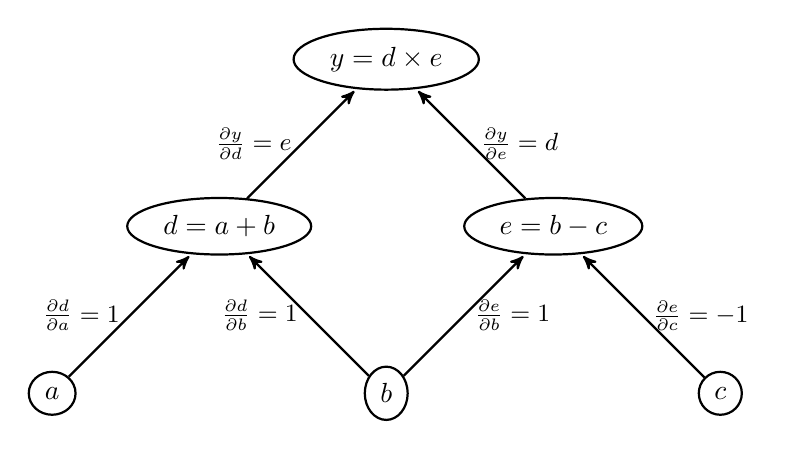
\begin{tikzpicture}[->,>=stealth',shorten >=1pt,auto,node distance=3cm,thick,main/.style={draw,ellipse,thick}]

      \node[main] (1) {$y = d \times e$};
      \node[main] (2) [below left of=1] {$d = a + b$};
      \node[main] (3) [below right of=1] {$e = b - c$};
      \node[main] (4) [below left of=2] {$a$};
      \node[main] (5) [below right of=2] {$b$};
      \node[main] (6) [below right of=3] {$c$};
      
      \path[every node/.style={font=\sffamily\small}]
      (2) edge node [left] {$\frac{\partial y}{\partial d}=e$} (1)
      (3) edge node [right] {$\frac{\partial y}{\partial e}=d$} (1)
      (4) edge node [left] {$\frac{\partial d}{\partial a}=1$} (2)
      (5) edge node [left] {$\frac{\partial d}{\partial b}=1$} (2)
          edge node [right] {$\frac{\partial e}{\partial b}=1$} (3)
      (6) edge node [right] {$\frac{\partial e}{\partial c}=-1$} (3);
    \end{tikzpicture}
    \caption{Computation Graph for $y = (a + b) \times (b - c)$}
    \label{fig:cg}
  \end{figure}
\end{center}

Applying the chain rule and collecting the derivatives along the edges of the graph, we can assemble
the (forward) derivatives of $y$ w.r.t. the input variables $a, b, c$
\begin{align*}
  \frac{\partial y}{\partial a} &= \frac{\partial y}{\partial d} \cdot \frac{\partial d}{\partial a} = e\\ 
  \frac{\partial y}{\partial b} &= \frac{\partial y}{\partial d} \cdot \frac{\partial d}{\partial b} +  \frac{\partial y}{\partial e} \cdot \frac{\partial e}{\partial b} = e + d \\
  \frac{\partial y}{\partial c} &= \frac{\partial y}{\partial e} \cdot \frac{\partial e}{\partial c} = -d
  \end{align*}

The following section provides a brief introduction to the AD mechanics, {\em Forward} and {\em Backward} modes. The latter is also referred to as Adjoint Algorithmic Differentiation (AAD) and particularly important for fast sensitivity calulation.

%------------------------------------------------------------------------------------------------------------
\subsection{Automatic Differentiation Basics}
%------------------------------------------------------------------------------------------------------------
\label{sec:ad}

Consider the evaluation of some function $y=f(x_1, ...., x_n)$ of $n$
input variables (e.g. an instrument value as a function of many market
data points).  Any such function evaluation can be expressed in terms
of $m$ intermediate variables to which we apply simple unary built-in 
functions (such as $\exp(x)$, $\log(x)$, $\sin(x)$, ...) and binary 
operations (addition, subtraction, multiplication, division).  

AD is a ``mechanical'' application of the chain rule of differentiation
% $$
% \frac{\partial y}{\partial x_j} = \sum_{k=1}^m
% \frac{\partial y}{\partial g_k}\frac{dg_k}{dx_j} 
% $$
to the series of intermediate results. The sequence can be evaluated
in two ways, forward and backward direction, as well as combinations of
both. The following sections sketch these procedures.

\subsection*{Forward Mode}

The concept of this mode is the one that is easier to understand. 
We assume that our functions do not operate on real numbers but on
{\em dual numbers} $x+\epsilon x'$ with an arithemtic defined by $\epsilon^2=0$.  
Basic operations -- addition, subtraction, multiplication, division of dual numbers
-- follow from this definition as
\begin{align*}
(x+\epsilon x') \pm (y+\epsilon y') &= x \pm y + \epsilon(x'\pm y') \\
(x+\epsilon x') \times (y+\epsilon y') &= x\,y + \epsilon(xy' +x'y) \\
%(y+\epsilon y') \times (y-\epsilon y') &= y^2 \\
 (x+\epsilon x') / (y+\epsilon y') &=
\frac{ (x+\epsilon x') \times (y-\epsilon y')}{(y+\epsilon y')\times
  (y-\epsilon y')} 
%= \frac{xy + \epsilon(x'y-y'x)}{y^2+\epsilon(y'y-y'y)}\\
= \frac{xy + \epsilon(x'y-y'x) }{y^2} \\
&= x/y + \epsilon(x'/y-y'x/y^2)
\end{align*}
Function evaluations of dual arguments follow from their truncated Taylor
expansion\footnote{Assuming that the derivative $f'(x)$ exists.} 
(as all powers $\epsilon^2, \epsilon^3, \dots$ vanish):
\begin{align*}
f(x+\epsilon x') &= f(x) + \epsilon\,f'(x)\,x'
\intertext{which also yields the chain rule}
f(g(x+\epsilon x')) &= f(g(x) + \epsilon\,g'(x)\,x') \\
&= f(g(x)) + \epsilon\,f'(g(x))\,g'(x)\,x'
\end{align*}
by iterated application of the first truncated Taylor series.
For $x'=1$ the RHS of the latter is just the derivative of $f(\cdot)$
w.r.t. $x$. All we need to do is generalize all operations to {\em
  dual numbers} and evaluate $f(g(x+\epsilon))$. This yields the usual
``primal'' valuation $f(g(x))$ and the function's derivative
mechanically by looking up the $\epsilon$ coefficient (second component)
of the resulting dual number. 

Generalizing to functions of $n$ variables $x_1, ..., x_n$, and their
dual generalization $(x_i+\epsilon x'_i)$, the 
difference is in the truncated Taylor expansion for the function
evaluations
$$
f(x_1+\epsilon x'_1,\dots,x_n+\epsilon x'_n) = f(x_1,\dots,x_n)
+\epsilon \sum_{i=1}^n \frac{\partial f}{\partial x_i} x'_i.
$$
This shows that we get any first order partial derivative by setting its {\em
  seed} $x'_i$ to one and all others to zero. Hence this forward mode
requires $n$ passes / valuations to get all $n$ partial derivatives.
The forward mode is efficient if we need to evaluate many functions
$f$ of few variables.

In finance it is often the other way around, few
functions need sensitivity calculation w.r.t. many input variables. 
The {\em backward} mode, sketched in the following, is 
suited for this situation.

\subsection*{Backward Mode, Adjoint Algorithmic Differentiation (AAD)}
\index{adjoint algorithmic differentiation|(textbf}
The backward mode evaluates the chain rule along
intermediate calculation steps in {\em reverse} order.
Consider a sequence of evaluations \cite{capriotti_2011c}
$$
X \rightarrow ... \rightarrow U \rightarrow V \rightarrow
... \rightarrow Y
$$  
which transforms the input $X$ (of dimension $n$) to the outptut $Y$
(of dimension $m$) using basic arithmetic operations and simple
built-in function calls for which the derivative is built-in as well. 
We are interested in all partial derivatives
$$
\frac{\partial Y_i}{\partial X_j}.
$$
The derivative of the function $Y: \R^n \to \R^m, X\mapsto Y(X)$ in $\xi\in\R^n$ is a linear operator $DY(\xi): \R^n\to\R^m$ which maps
$$
\left(\begin{matrix}
x_1\\ 
\vdots\\ 
x_n
\end{matrix}\right)
 \mapsto 
\left( \begin{matrix}
\frac{\partial Y_1}{\partial X_1}(\xi) & \cdots & \frac{\partial Y_1}{\partial X_n}(\xi)\\
\vdots & \ddots & \vdots\\
\frac{\partial Y_m}{\partial X_1}(\xi) & \cdots & \frac{\partial Y_m}{\partial X_n}(\xi)
\end{matrix}\right) \!
\left(\begin{matrix}
x_1\\ 
\vdots\\ 
x_n
\end{matrix}\right)
= \left(\begin{matrix}
\sum_{i=1}^n \frac{\partial Y_1}{\partial X_i}(\xi)\,x_i\\ 
\vdots\\ 
\sum_{i=1}^n \frac{\partial Y_m}{\partial X_i}(\xi)\,x_i\\ 
\end{matrix}\right) \!.$$
Because all variables are real, the adjoint operator of $DY(\xi)$ is
$$(DY(\xi)^* = \left( \begin{matrix}
\frac{\partial Y_1}{\partial X_1}(\xi) & \cdots & \frac{\partial Y_1}{\partial X_n}(\xi)\\
\vdots & \ddots & \vdots\\
\frac{\partial Y_m}{\partial X_1}(\xi) & \cdots & \frac{\partial Y_m}{\partial X_n}(\xi)
\end{matrix}\right)^{\top} \!= 
\left( \begin{matrix}
\frac{\partial Y_1}{\partial X_1}(\xi) & \cdots & \frac{\partial Y_m}{\partial X_1}(\xi)\\
\vdots & \ddots & \vdots\\
\frac{\partial Y_1}{\partial X_n}(\xi) & \cdots & \frac{\partial Y_m}{\partial X_n}(\xi)
\end{matrix}\right).
$$
For intermediate functions, the chain rule in conjunction with the multiplication rule for transposed matrices yields:
\begin{align*}
Y(X) &= Y(V(X)) \Rightarrow\\
(DY(\xi))^* &= (DY(V(\xi))\,DV(\xi))^* \\
&= (DV(\xi))^*\,(DY(V(\xi)))^*
\end{align*}
which allows us to compute the derivatives backwards, provided we can compute the adjoint operators. 
Hence, the backward mode considers {\em adjoint} variables
$$
\bar V_k = \sum_{j=1}^m \bar Y_j \frac{\partial Y_j}{\partial V_k}
$$ 
which collect the sensitivity of the result w.r.t. intermediate 
variable $V_k$. Likewise
$$
\bar U_i = \sum_{j=1}^m \bar Y_j \frac{\partial Y_j}{\partial U_i} 
= \sum_{j=1}^m \bar Y_j \sum_k \frac{\partial Y_j}{\partial
  V_k}\frac{\partial V_k}{\partial U_i} 
= \sum_k \bar V_k \frac{\partial V_k}{\partial U_i}
$$
Starting from the adjoint of the output we can eventually generate the
adjoint of the input variables 
\begin{align}
  \label{eq_adjoint_der_op}
\bar X_i & = \sum_{j=1}^m \bar Y_j \frac{\partial Y_j}{\partial X_i} 
\end{align}
by applying the chain rule to all intermediate results in reverse
order
$$
\bar X \leftarrow ... \leftarrow \bar U \leftarrow \bar V \leftarrow
... \leftarrow \bar Y.
$$  
Initializing the output adjoint for index $j$ with one (and all other
with zero) in \eqref{eq_adjoint_der_op} therefore yields the entire set of sensitivities of $Y_i$
to all $n$ input variables. Due to the formulation in terms of 
adjoint variables, AD in backward mode is also referred to as {\em Adjoint Algorithmic Differentiation
  (AAD)}.
Recall that the overall complexity of sensitivity calculation using AAD is no more than
four times greater than the complexity (in terms of number of operations) 
of the original valuation. The general rule is: The adjoint method should be used in case there
are many inputs (curve points, volatilities, credit spreads etc.) but few outputs (prices,
value adjustments). If there are few inputs but many outputs, the forward method is better.
 
\medskip
Note that the reverse procedure uses
partial derivatives of internal variables $V_k$ w.r.t. internal
variables $U_i$ which are generally dependent on the values of
internal variables. This means they need to be computed in a first
forward {\em sweep} and then stored for usage in the backward sweep.
This memory impact is different from the pure forward sweep which
does not require storing intermediate results.

\subsection{Computation Graphs in ORE}

{\em Operator Overloading} is a typical approach to ``recording'' a computation graph automatically.
See for example the attempts to integrate AAD with Operator Overloading into QuantLib \cite{QuantLib}
around 2014. See also the series of papers by Antoine Savine on the subject \cite{savine_cg_1,
  savine_cg_2, savine_cg_3} and his books for a deeper dive \cite{savine_book_1, savine_book_2}.

However, in ORE we apply AAD in the context of the scripted trade module only. Rather than following
the operator overloading path introducing an ``active'' {\tt Real} data type, replacing the
``inactive'' {\tt Real} type across the entire ORE libraries, we extract the computation graph
explicitly from the script in its AST representation in order to utilize AAD in the scripted trade
processing only. Thus we avoid negative perfomance impact (recall the ``factor 4'' overhead)
elsewhere and in the valuation of vanilla instruments. Moreover, we make the ``AAD activation'' of the
scripted trade framework configurable, i.e. we can switch AAD on and off without recompiling the
code base. How this works is discussed briefly in the following.

The {\tt ComputationGraph} object is defined in qle/math/ad/computationgraph.*pp, alongside
essential operations on the graph -- forward valuation, forward and backward derivative propagation.
It is recommended to review the compact implementation of the these functions in qle/math/ad,
see listings \ref{lst:forwardvaluation}, \ref{lst:forwardderivatives} and \ref{lst:backwardderivatives}.

\begin{listing}[hbt]
\begin{minted}[fontsize=\scriptsize]{c++}
template <class T>
void forwardEvaluation(const ComputationGraph& g, std::vector<T>& values,
                       const std::vector<std::function<T(const std::vector<const T*>&)>>& ops,
                       std::function<void(T&)> deleter = {}, bool keepValuesForDerivatives = true,
                       const std::vector<std::function<std::pair<std::vector<bool>, bool>(const std::size_t)>>&
                           opRequiresNodesForDerivatives = {},
                       const std::vector<bool>& keepNodes = {}, const std::size_t startNode = 0,
                       const std::size_t endNode = ComputationGraph::nan, const bool redBlockReconstruction = false) {

    std::vector<bool> keepNodesDerivatives;
    if (deleter && keepValuesForDerivatives)
        keepNodesDerivatives = std::vector<bool>(g.size(), false);

    // loop over the nodes in the graph in ascending order

    for (std::size_t node = startNode; node < (endNode == ComputationGraph::nan ? g.size() : endNode); ++node) {

        // if a node is computed by an op applied to predecessors ...
        if (!g.predecessors(node).empty()) {

            // evaluate the node

            std::vector<const T*> args(g.predecessors(node).size());
            for (std::size_t arg = 0; arg < g.predecessors(node).size(); ++arg) {
                args[arg] = &values[g.predecessors(node)[arg]];
            }
            values[node] = ops[g.opId(node)](args);

            QL_REQUIRE(values[node].initialised(), "forwardEvaluation(): value at active node "
                                                   << node << " is not initialized, opId = " << g.opId(node));

            // then check if we can delete the predecessors
            if (deleter) {
                ...
            }     // if deleter
        }         // if !g.predecessors empty
    }             // for node
}
\end{minted}
\caption{Forward valuation on a computation graph in qle/ad/forwardvaluation.hpp}
\label{lst:forwardvaluation}
\end{listing}

\begin{listing}
\begin{minted}[fontsize=\scriptsize]{c++}
template <class T>
void forwardDerivatives(const ComputationGraph& g, const std::vector<T>& values, std::vector<T>& derivatives,
                        const std::vector<std::function<std::vector<T>(const std::vector<const T*>&, const T*)>>& grad,
                        std::function<void(T&)> deleter = {}, const std::vector<bool>& keepNodes = {},
                        const std::size_t conditionalExpectationOpId = 0,
                        const std::function<T(const std::vector<const T*>&)>& conditionalExpectation = {}) {

    if (g.size() == 0)
        return;

    // loop over the nodes in the graph in forward order

    for (std::size_t node = 0; node < g.size(); ++node) {
        if (!g.predecessors(node).empty()) {

            // propagate the derivatives from predecessors of a node to the node

            std::vector<const T*> args(g.predecessors(node).size());
            for (std::size_t arg = 0; arg < g.predecessors(node).size(); ++arg) {
                args[arg] = &values[g.predecessors(node)[arg]];
            }

            if (g.opId(node) == conditionalExpectationOpId && conditionalExpectation) {

                args[0] = &derivatives[g.predecessors(node)[0]];
                derivatives[node] = conditionalExpectation(args);

            } else {

                auto gr = grad[g.opId(node)](args, &values[node]);

                for (std::size_t p = 0; p < g.predecessors(node).size(); ++p) {
                    derivatives[node] += derivatives[g.predecessors(node)[p]] * gr[p];
                }
            }

            // the check if we can delete the predecessors

            if (deleter) {
                ...  
            }     // if deleter
        }         // if !g.predecessors empty
    }             // for node
}
\end{minted}
\caption{Forward derivaties calculation on a computation graph in qle/ad/forwardderivatives.hpp}
\label{lst:forwardderivatives}
\end{listing}

\begin{listing}
\begin{minted}[fontsize=\scriptsize]{c++}
template <class T>
void backwardDerivatives(const ComputationGraph& g, std::vector<T>& values, std::vector<T>& derivatives,
                         const std::vector<std::function<std::vector<T>(const std::vector<const T*>&, const T*)>>& grad,
                         std::function<void(T&)> deleter = {}, const std::vector<bool>& keepNodes = {},
                         const std::vector<std::function<T(const std::vector<const T*>&)>>& fwdOps = {},
                         const std::vector<std::function<std::pair<std::vector<bool>, bool>(const std::size_t)>>&
                             fwdOpRequiresNodesForDerivatives = {},
                         const std::vector<bool>& fwdKeepNodes = {}, const std::size_t conditionalExpectationOpId = 0,
                         const std::function<T(const std::vector<const T*>&)>& conditionalExpectation = {}) {

    if (g.size() == 0)
        return;

    std::size_t redBlockId = 0;

    // loop over the nodes in the graph in reverse order

    for (std::size_t node = g.size() - 1; node > 0; --node) {

        if (g.redBlockId(node) != redBlockId) {

            // delete the values in the previous red block
            ...

            // populate the values in the current red block
            ...

            // update the red block id
            redBlockId = g.redBlockId(node);
        }

        if (!g.predecessors(node).empty() && !isDeterministicAndZero(derivatives[node])) {

            // propagate the derivative at a node to its predecessors
            std::vector<const T*> args(g.predecessors(node).size());
            for (std::size_t arg = 0; arg < g.predecessors(node).size(); ++arg) {
                args[arg] = &values[g.predecessors(node)[arg]];
            }

            QL_REQUIRE(derivatives[node].initialised(),
                       "backwardDerivatives(): derivative at active node " << node << " is not initialized.");

            if (g.opId(node) == conditionalExpectationOpId && conditionalExpectation) {

                // expected stochastic automatic differentiaion, Fries, 2017
                args[0] = &derivatives[node];
                derivatives[g.predecessors(node)[0]] += conditionalExpectation(args);

            } else {

                auto gr = grad[g.opId(node)](args, &values[node]);

                for (std::size_t p = 0; p < g.predecessors(node).size(); ++p) {
                    ...
                    derivatives[g.predecessors(node)[p]] += derivatives[node] * gr[p];
                }
            }
        }

        // then check if we can delete the node
        ...

    } // for node
}
\end{minted}
\caption{Backward derivaties calculation on a computation graph in qle/ad/backwardderivatives.hpp}
\label{lst:backwardderivatives}
\end{listing}

To utilise the computation graph, ORE provides an additional hierarchy of scripting models and
engines, as well as a configuration graph builder using the AST, summarized in table \ref{tab:cg}.
Which side of the hierarchy is built, depends on configuration settings in pricingengine.xml
(UseCG, UseAD). We can use the computation graph version even without activating AD.

\begin{table}[htb]
  \scriptsize
  \begin{tabular}{|l|l|}
    \hline
    models/model.hpp &
    models/model{\color{red}cg}.*pp \\
    models/modelimpl.*pp &
    models/model{\color{red}cg}impl.*pp \\
    models/blackscholes.hpp &
    models/blackscholes{\color{red}cg}.*pp \\
    models/blackscholesbase.*pp &
    models/blackscholes{\color{red}cg}base.*pp \\
    models/gaussiancam.*pp &
    models/gaussiancam{\color{red}cg}.*pp \\
    models/localvol.*pp & -- \\
    -- & models/hw{\color{red}cg}.*pp \\
    -- & models/lgm{\color{red}cg}.*pp \\
    \hline
    engines/scriptedinstrumentpricingengine.*pp &
    engines/scriptedinstrumentpricingengine{\color{red}cg}.*pp \\
    \hline
    -- & computationgraphbuilder.*pp \\
    \hline
\end{tabular}
\caption{``Classic'' scripting vs ``Computation Graph'', all files is ore/scripting.}
\label{tab:cg}
\end{table}

Apparently these implementation have somewhat different scope (see localvol on the ``classic'' side,
hwcg, and lgmcg on the ``CG'' side), which shows that the module is
still in progress, on both sides with and without computation graph utilisation.
Generally the duplication of code here (about 3500 lines of code in the models and engine
classes of type CG) seems undesireable, disadvantageous from a development and maintenance effort
point of view.

However, our plan is to continue following and building out the computation graph
path (adding more scripting models over time) and to keep the ``classic'' implementation available
for validation and testing for part of the computation graph framework.

Key differences:
\begin{itemize}
\item {\tt ScriptedInstrumentPricingEngineCG} calls the {\tt ComputationGraphBuilder} which
  constructs the computation graph from the AST and delegates the pricing to the
  {\tt forwardEvaluatiuon} function defined in qle/ad that operates on the computation graph;
  it does {\em not} use the {\tt ASTRunner} any more
\item the scripting models, starting with base class {\tt ModelCG}, have a similar interface as
  the ``non-CG'' counterparts with {\tt RandomVariable} arguments replaced with indexes (of type
  std::size\_t) referencing nodes in the computation graph, see the cut-down listing of
  {\tt ModelCG} in listing \ref{lst:modelcg} and compare to the {\tt Model} interface in
  listing  \ref{lst:model}; the scripting model classes provide additional
  member functions that reference random variates and model parameters on the graph;
\end{itemize}

\begin{listing}
\begin{minted}[fontsize=\scriptsize]{c++}
class ModelCG : public QuantLib::LazyObject {
public:
    enum class Type { MC, FD };

    explicit ModelCG(const QuantLib::Size n);

    // computation graph
    boost::shared_ptr<QuantExt::ComputationGraph> computationGraph() { return g_; }

    // result must be as of max(refdate, obsdate); refdate < paydate and obsdate <= paydate required
    virtual std::size_t pay(const std::size_t amount, const Date& obsdate, const Date& paydate,
                            const std::string& currency) const = 0;

    // refdate <= obsdate <= paydate required
    virtual std::size_t discount(...)

    // refdate <= obsdate required
    virtual std::size_t npv(const std::size_t amount, const Date& obsdate, const std::size_t filter,
                            const boost::optional<long>& memSlot, const std::size_t addRegressor1,
                            const std::size_t addRegressor2) const = 0;
    ...

    // CG / AD part of the interface
    virtual std::size_t cgVersion() const = 0;
    virtual const std::vector<std::vector<std::size_t>>& randomVariates() const = 0; 
    virtual std::vector<std::pair<std::size_t, double>> modelParameters() const = 0;
    ...
 };
\end{minted}
\caption{Scripting model base class {\tt ModelCG} using a computation graph.}
\label{lst:modelcg}
\end{listing}

%-----------------------------------------------------------------------------------------------------
\subsection{NPV Sensitivities with AAD}
%-----------------------------------------------------------------------------------------------------

Now we can utilise the backward sensitivity calculation on the computation graph to compute
trade/portfolio sensitivities (for scripted trades). All we need to do for that purpose -- as a user
of ORE -- is providing a scripted trade pricing engine configuration of the kind in listing
\ref{lst:pricingengineconfig_aad}.

\begin{listing}[hbt]
\begin{minted}[fontsize=\scriptsize]{xml}
<PricingEngines>
  <Product type="ScriptedTrade">
    <Model>Generic</Model>
    <ModelParameters>
      <Parameter name="Model">GaussianCam</Parameter>
      ...
    </ModelParameters>
    <Engine>Generic</Engine>
    <EngineParameters>
      <Parameter name="Engine">MC</Parameter>
      <Parameter name="Samples">8192</Parameter>
      <Parameter name="RegressionOrder">4</Parameter>
      <Parameter name="TimeStepsPerYear">1</Parameter>
      <Parameter name="Interactive">false</Parameter>
      <Parameter name="BootstrapTolerance">1.0</Parameter>
      <Parameter name="ZeroVolatility">false</Parameter>
      <Parameter name="Interactive">false</Parameter>
      <Parameter name="UseAD">true</Parameter>
    </EngineParameters>
  </Product>
</PricingEngines>
\end{minted}
\caption{Scripted Trade pricing engine configuration to generate AAD sensitivities: {\tt UseAD=true}.}
\label{lst:pricingengineconfig_aad}
\end{listing}

i.e. with {\tt Engine} set to MC and {\tt UseAD} flag set to true.
This triggers the construction of the computation graph version of scripting models and script engine.

When we run the usual pricing/sensitivity analytic in ORE, this will cause the generation of
backward sensitivities in the first pricing call, and sensitivities are cached as pricing
engine additional results, see upper half of listing \ref{lst:sensicache}.
When we then run the usual bump \& revalue sensitivity scenarios and
reprice the instrument repeatedly, then we read the cached sensitivities, scale them to the
desired bump size and populate the sensitivity cube, see lower half of listing \ref{lst:sensicache}.
This is fully integrated with the rest of the portfolio represented as ``classic'' trades.

\begin{listing}[hbt]
\begin{minted}[fontsize=\scriptsize]{c++}
void ScriptedInstrumentPricingEngineCG::calculate() const {
    ...
    if (!haveBaseValues_ || !useCachedSensis_) {
        ...
        if (useCachedSensis_) {

            // extract sensis and store them

            std::vector<RandomVariable> derivatives(g->size(), RandomVariable(model_->size(), 0.0));
            derivatives[cg_var(*g, npv_ + "_0")] = RandomVariable(model_->size(), 1.0);
            backwardDerivatives(*g, values, derivatives, grads_, RandomVariable::deleter, keepNodes);

            sensis_.resize(baseModelParams_.size());
            for (Size i = 0; i < baseModelParams_.size(); ++i) {
                sensis_[i] = model_->extractT0Result(derivatives[baseModelParams_[i].first]);
            }
            DLOG("got backward sensitivities");

            // set flag indicating that we can use cached sensis in subsequent calculations

            haveBaseValues_ = true;
        }

    } else {

        // useCachedSensis => calculate npv from stored base npv, sensis, model params

        auto modelParams = model_->modelParameters();

        double npv = baseNpv_;
        DLOG("computing npv using baseNpv " << baseNpv_ << " and sensis.");

        for (Size i = 0; i < baseModelParams_.size(); ++i) {
            QL_REQUIRE(...)
            Real tmp = sensis_[i] * (modelParams[i].second - baseModelParams_[i].second);
            npv += tmp;
            DLOG(...)
        }
        results_.value = npv;
    }
    ...
}
\end{minted}
\caption{Scripted Instrument Pricing Engine CG - this excerpt shows the caching of backward
  sensitivities upon the first pricing call (upper part), as well as their utilisation on subsequent
  calls to simulate NPVs in line with base NPV, sensitivities and risk factor bump sizes.}
\label{lst:sensicache}
\end{listing}


%-----------------------------------------------------------------------------------------------------
\subsection{XVA Sensitivities with AAD}
%-----------------------------------------------------------------------------------------------------

The XVA sensitivity calculation using AAD is in development in ORE and in an experimental,
proof of concept state at the time of writing this text.

ORE Example 56 demonstrates the current functionality using ORE's command line interface.
Note that interface and implementation details are subject to change.

The key idea is to reuse ORE's ComputationGraph in the scripted trade framework.
The case in Example 56 is particularly simple, a single Swap.

The AAD XVA sensitivity calculation is triggered in ore.xml as shown in listing
\ref{lst:orexml_xva_sensi_aad}, i.e. with parameters
\begin{itemize}
\item amc set to true, so that we run the exposure calculation with AMC
\item amcCg set to true, so that we call a new {\tt XvaEngineCG} (defined in
  orea/engine/xvaenginecg.*pp) that has the capability to generates both XVA and XVA sensitivities,
  when running the XVA analytic
\item xvaSensitivityConfig set to a valid sensitivity config file
\end{itemize}

\begin{listing}[hbt]
\begin{minted}[fontsize=\scriptsize]{xml}
    <Analytic type="simulation">
      <Parameter name="active">true</Parameter>
      <Parameter name="amc">true</Parameter>
      <Parameter name="amcCg">true</Parameter>
      <Parameter name="xvaCgSensitivityConfigFile">xvasensiconfig.xml</Parameter>
      <Parameter name="amcTradeTypes">Swap</Parameter>
      <Parameter name="amcPricingEnginesFile">pricingengine_amc.xml</Parameter>
      ...
    </Analytic>
\end{minted}
\caption{ore.xml settings for XVA sendsitivity calculation using AAD: {\tt amc=true},
  {\tt amcCg=true}, {\tt xvaCgSensitivityConfigFile} set.}
\label{lst:orexml_xva_sensi_aad}
\end{listing}

Moreover, we need to set {\tt UseCG} set to {\tt true} in the pricing engine configuration
\ref{lst:pricignengine_xva_sensi_aad} used in the simulation phase,
so that we build the trade using the computation graph scripting models.

\begin{listing}[hbt]
\begin{minted}[fontsize=\scriptsize]{xml}
  <Product type="ScriptedTrade">
    <Model>Generic</Model>
    <ModelParameters>
      <Parameter name="Model">GaussianCam</Parameter>
      ...
    </ModelParameters>
    <Engine>Generic</Engine>
    <EngineParameters>
      <Parameter name="Engine">MC</Parameter>
      <Parameter name="UseCG">true</Parameter>
      ...
    </EngineParameters>
  </Product>
\end{minted}
\caption{pricingengine.xml for XVA sensitivity calculation using AAD: {\tt UseCG=true}.}
\label{lst:pricignengine_xva_sensi_aad}
\end{listing}

When running the XvaAnalytic with the settings above, we will bypass the usual process
and call into a new analytic {\tt XvaAnalyticCG} defined in orea/engine/xvaenginecg.*pp,
as shown in listing \ref{lst:xvaenginecg}.

\begin{listing}[hbt]
\begin{minted}[fontsize=\scriptsize]{c++}
void XvaAnalyticImpl::runAnalytic(const boost::shared_ptr<ore::data::InMemoryLoader>& loader,
                              const std::set<std::string>& runTypes) {
    if(inputs_->amcCg()) {
        LOG("XVA analytic is running with amc cg engine (experimental).");
        XvaEngineCG engine(
            inputs_->nThreads(), inputs_->asof(), loader, inputs_->curveConfigs().get(),
            analytic()->configurations().todaysMarketParams, analytic()->configurations().simMarketParams,
            inputs_->amcPricingEngine(), inputs_->crossAssetModelData(), inputs_->scenarioGeneratorData(),
            inputs_->portfolio(), inputs_->marketConfig("simulation"), inputs_->marketConfig("simulation"),
            inputs_->xvaCgSensiScenarioData(), inputs_->refDataManager(), *inputs_->iborFallbackConfig());
        return;
    }
\end{minted}
\caption{Call into the experimental XVA AAD-Sensitivity implementation, bypassing the ususal XVA run.}
\label{lst:xvaenginecg}
\end{listing}

This new analytic covers the following steps
\begin{itemize}
\item build today's market
\item build a simulation market
\item build the {\tt GaussianCamCG} scripting model
\item build the portfolio against the latter
\item build the computation graph for all trades
\item add nodes to the computation graph which sum the exposure over trades
\item add nodes for the CVA calculation
\item run a forward evaluation
\item write exposure reports
\item compute CVA as expectation over random variable values in the CVA node
\item do a backward derivatives run
\item fill the sensitivity cube by copying the AAD derivatives (or do repeated forward valuations for bump sensitivities);
  this is currently controlled by a hard-coded boolean {\tt bumpCvaSensis}
\item write the sensitivity report
\end{itemize}

i.e. it replaces the entire XVA analytic and the post processing of the NPV cube.

For testing/validation purposes (accuracy of results, performance) we can activate bump \& revalue sensitivity
calculation by setting the hard coded boolean {\tt bumpCvaSensis=true} in orea/engine/xvaenginecg.cpp.

%------------------------------------------------------------------------------------------------------------
\section{External Compute Devices}
%------------------------------------------------------------------------------------------------------------

In the application of ORE at industrial scale we occasionally hit cases where the performance of
an ORE based service is not sufficient to keep processing times within agreed limits. One example
are backtesting runs for particularly complex portfolios (including Accumulators and TaRFs) which
require the repricing of the portfolio on several thousand market scenarios.

ORE's multi-threaded valuation engine helps utilising the available CPU cores, but the speed-up we
can achieve with multi-threading in ORE is limited by the typically low number of cores and also
the overhead in setting up markets and portfolios for each thread. The speed-ups we have achieved
with multi-threading on our available hardware has been well below factor 10 so far.

Thanks to the growing popularity of AI tools and need for machine learning infrastructure graphics
cards with hundreds of GPU cores have become more broadly available. One can easily rent AWS
hardware with A100 Nvidia cards nowadays. Moreover, compiler support for such hardware has much improved
over the past ten years. So it is time to utilise such devices with ORE to
cut down run times by orders of magnitude where required by an SLA.

The computation graph representation of a scripted trade is also suited to build a particularly slim
interface to an external compute device (GPU), because the computation graph is a very
low level ``atomic'' representation of the algorithms we need to run. The idea is
\begin{itemize}
\item to compile the processing of a computation graph into a GPU kernal
\item to run the computation graph multiple (thousands of) times with changing context
\item to minimise the amount of data exchange between CPU and GPU
\end{itemize}

To support external devices, ORE provides a compute framework interface, defined in
see qle/math/computeenvironment.*pp. This contains three class declarations, two of which (the latter two)
need to be implemented in derived classes, see listings \ref{lst:computecontext} and
\ref{lst:computeframework}
\begin{itemize}
\item {\tt ComputeEnvironment}: A thread-local singleton that exposes external compute frameworks to ORE. A new framework has to be registered to this singleton.
\item {\tt ComputeFramework}
\item {\tt ComputeContext} 
\end{itemize}

\begin{listing}[hbt]
\begin{minted}[fontsize=\scriptsize]{c++}
class ComputeFramework {
public:
    virtual ~ComputeFramework() {}
    virtual std::set<std::string> getAvailableDevices() const = 0;
    virtual ComputeContext* getContext(const std::string& deviceName) = 0;
};
\end{minted}
\caption{Compute framework, provides the Compute Context for each device.}
\label{lst:computeframework}
\end{listing}

\begin{listing}[hbt]
\begin{minted}[fontsize=\scriptsize]{c++}
class ComputeContext {
public:
    ...
    virtual std::pair<std::size_t, bool> initiateCalculation(const std::size_t n,
                                                             const std::size_t id = 0,
                                                             const std::size_t version = 0,
                                                             const bool debug = false) = 0;
    virtual std::size_t createInputVariable(double v) = 0;
    virtual std::size_t createInputVariable(double* v) = 0;
    virtual std::vector<std::vector<std::size_t>> createInputVariates(const std::size_t dim,
                                                                      const std::size_t steps,
                                                                      const std::uint32_t seed) = 0;
    virtual std::size_t applyOperation(const std::size_t randomVariableOpCode,
                                       const std::vector<std::size_t>& args) = 0;
    virtual void freeVariable(const std::size_t id) = 0;
    virtual void declareOutputVariable(const std::size_t id) = 0;

    virtual void finalizeCalculation(std::vector<double*>& output, const Settings& settings) = 0;

    ...    
};
\end{minted}
\caption{The context in which calculations can be performed. The {\tt ComputeFramework} provides a pointer
  to the {\tt ComputeContext} for each device.}
\label{lst:computecontext}
\end{listing}

Review the technical documentation for the compute environment interface in Docs/ComputeEnvironment
at \url{https://github.com/OpenSourceRisk/Engine}.

This interface is not tied to the scripted trade framework in principle. But so far the only use
case in ORE is linked to the scripted trade framework with computation graph: In order to utilise an
external device with ORE we need to set a few pricing engine parameters as shown in listing
\ref{lst:pricingengine_gpu}.

\begin{listing}[hbt]
\begin{minted}[fontsize=\scriptsize]{xml}
<PricingEngines>
  <Product type="ScriptedTrade">
    ...
    <EngineParameters>
      ...
      <Parameter name="UseCG">true</Parameter>
      <Parameter name="UseExternalComputeDevice">true</Parameter>
      <Parameter name="ExternalComputeDevice">OpenCL/Apple/AMD Radeon Pro 5500M Compute Engine</Parameter>
    </EngineParameters>
  </Product>
  ...
</PricingEngines>
\end{minted}
\caption{Pricing engine configuration for using an external device.}
\label{lst:pricingengine_gpu}
\end{listing}

So far there are two implementations of the ComputeContext that can be selected via the
{\tt ExternalComputeDevice} parameter
\begin{itemize}
\item a dummy implementation called ``BasicCpuContext'' which will utilise the CPU cores to do the work, see qle/math/basiccpuenvironment.*pp
\item an OpenCL reference implementation (in experimental state at the time of writing this text), see qle/math/openclenvironment.*pp
\end{itemize}
and a third implementation (CUDA) has been started. Both the OpenCL and CUDA implementations are
expected to be completed by the time of the 13th ORE release mid 2024.


%------------------------------------------------------------------------------------------------------------
\chapter{ORE Integration}
%------------------------------------------------------------------------------------------------------------

%------------------------------------------------------------------------------------------------------------
\section{Language Bindings}
%------------------------------------------------------------------------------------------------------------

To facilitate ORE adoption and integration it is useful to ``bind'' ORE with languages other
than C++, because C++ development familiarity is less widely spread than e.g. Python or Java.
Especially the younger generation of computer scientists are typically versatile in Python,
because of the vast landscape of Python packages that one gets easily with ``pip install ...'',
and perhaps in particular because of the popularity of machine learning and related Python tools
such as TensorFlow.

\subsection*{SWIG}

ORE language bindings are currently built using SWIG \cite{swig}, following the QuantLib example. 
The project is located in the separate repository \url{https://github.com/opensourcerisk/ore-swig}.

The initial goal of the ORE-SWIG project was to provide a working {\em framework} that allows building
{\em a single module} that provides access to classes and functions {\em across ORE and QuantLib}.
Primarily we wanted to be able to execute the following few lines in Python, in order to kick
off an ORE process.

\begin{minted}[fontsize=\scriptsize]{python}
from ORE import *
params = Parameters()
params.fromFile("Input/ore.xml")
ore = OREApp(params)
ore.run()
\end{minted}

The secondary goal was to access and manipulate underlying ORE and QuantLib objects that are assembled
during the OREApp.run() call. This is why we wanted to include QuantLib in our ORE module.

The QuantLib project has used SWIG for the purpose of wrapping QuantLib since the early 2000s,
because the team has been aiming for exposing QuantLib to many languages including Java, Python,
R and C\#. To utilise the existing wrapper code base of QuantLib we therefore decided to also adopt
the SWIG approach for ORE.

The main interest among ORE and QuantLib users in the industry seems to be in the Python
language bindings, although we also supported clients in using the Java module.
If we just wanted to wrap ORE classes into Python and abandon access to the underlying
QuantLib universe, then we would probably adopt a different framework such as boost.Python
(https://github.com/boostorg/python) to build the module.

\subsection*{Current Scope}

Since the first release of ORE-SWIG, ORE coverage has grown. However it is still patchy  
at about 11\% of the classes in ORE wrapped (about 200/1850, see appendix \ref{app:swig}),
compared to 44\% coverage in QuantLib (about 920/2100). 

As of today, users can query the {\tt OREApp} class and retrieve portfolio, market and underlying
term structures. Recently, while refactoring OREApp with
\begin{itemize}
\item separating analytics (see orea/app/analytics) 
\item ensuring results are kept primarily in-memory
\item results can be retrieved via an extended API from OREApp
\item separate file output of results on demand 
\item factoring out an input parameters object with API to set and get any member object
\item input data instance can be passed to OREApp
\end{itemize}
we have extended the OREApp API and added the InputParameters API to the SWIG wrapper,
for data management outside (before and after) calling {\tt ORE.run()} and to facilitate
ORE-based application development in Python.

We curently extend the SWIG wrapper scope mainly upon client request, rather than embarking
on a systematic internal extension project. 

\subsection*{Python Wheels}

A notable addition in 2023 was establishing a process of building Python {\em wheels} using github
actions post release. The wheels are published on the Python Package Index (PyPI) so that users can
install the latest ORE Python module for their platform conveniently using the command

\centerline{\tt pip install open-source-risk-engine}

again following the QuantLib example.

Similarly, we have added github actions to build ORE executables for Windows, macOS and
Linux platforms automatically on github after each update of the github master branch, keeping
the builds following a release, so that users can easily download the required executable and
explore ORE without going through the complex build process from C++ sources.

When using the ORE wheel with pip install, we recommend the following steps to isolate the ORE environment
\begin{minted}[fontsize=\scriptsize]{python}
python -m venv ore_env
source ore_env/bin/activate (.\ore_env\Scripts\activate.bat)
python -m pip install open-source-risk-engine
\end{minted}

\subsection*{Juyter Notebooks}

The public Python wheels also make various Jupyter notebooks readily accessible that are published
in the \url{https://github.com/opensourcerisk/ore-swig} repository's
OREAnalytics-SWIG/Python/Examples/Notebooks folder.
Juypter notebooks are convenient for prototyping ORE based applications, they can call into ORE,
retrieve results in memory for post-processing including visualisations in the notebook,
see a snapshot in figure \ref{fig:notebook}. Run the notebook in the same environment as above

\begin{minted}[fontsize=\scriptsize]{python}
python -m pip install jupyterlab
python -m jupyterlab &
\end{minted}

\begin{figure}[h]
\begin{center}
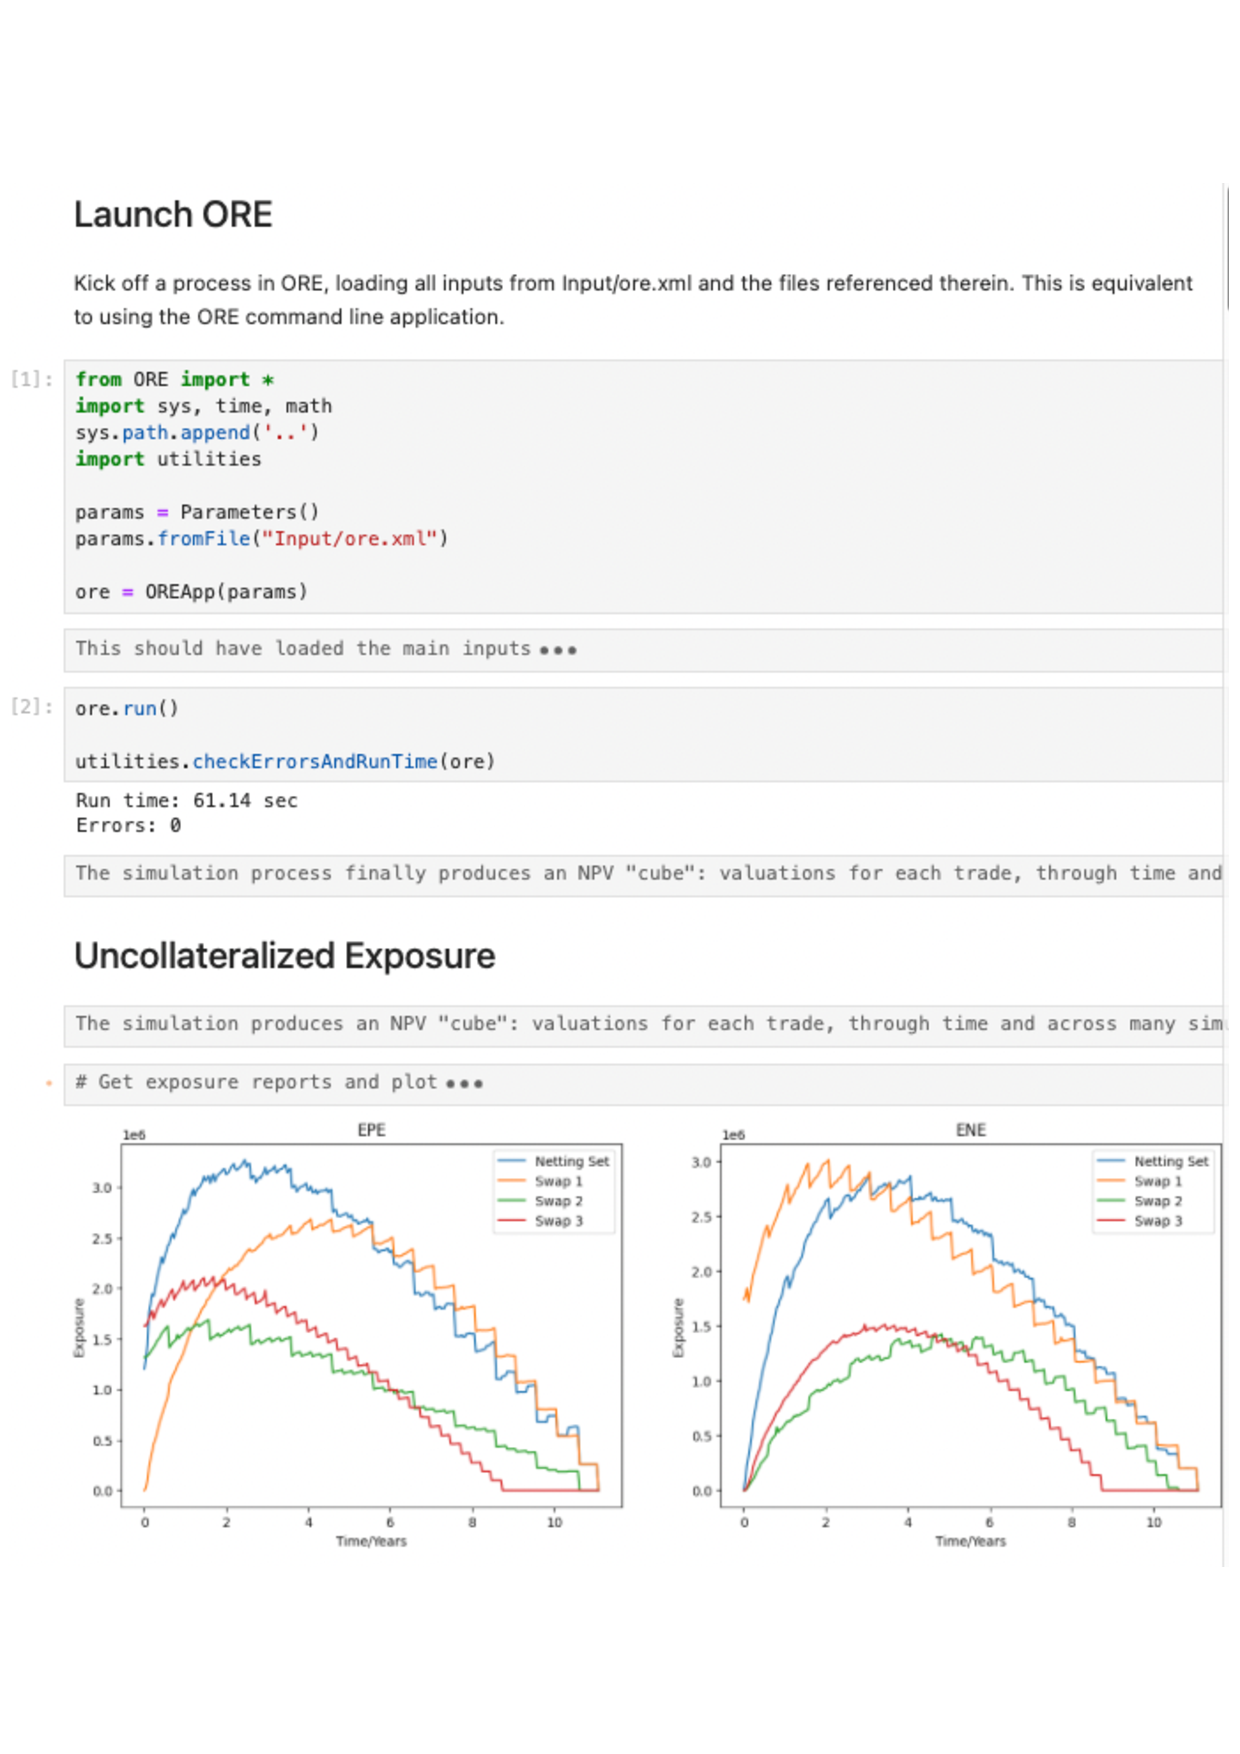
\includegraphics[scale=0.8]{data/notebook.pdf}
\end{center}
\caption{Jupyter notebook in OREAnalytics-SWIG/Python/Examples/Notebooks/Example\_2,
  calling ORE for generating collateralised exposures, retrieving results in memory for post-processing
  including visualisation in the notebook.}
\label{fig:notebook}
\end{figure}
\clearpage

\subsection*{Extending ORE SWIG}

Developing the ORE SWIG wrapper involves adding interface files (with ending *.i) in folders
\begin{itemize}
\item QuantExt-SWIG/SWIG
\item OREData-SWIG/SWIG
\item OREAnalytics-SWIG/SWIG
\end{itemize}
where we -- in a nutshell -- add a header for each class we want to expose, including the desired
subset of member function declarations. See any of the interface files in the folders above for examples
and compare C++ class declarations to the interface definition in the *.i file.
The {\tt README.md} at \url{https://github.com/opensourcerisk/ore-swig} then provides links to
tutorials for building the bindings and building Python wheels.

Extending the interface is simple in principle, but it is typically a slow and iterative process, because
\begin{itemize}
\item compilation time is long since the SWIG-generated C++ source file is particularly large (it covers all
  libraries - QuantLib, QuantExt, OREData and OREAnalytics)
\item namespace conflicts occur regularly because all objects are imported from the QuantLib, QuantExt, ore::data,
  ore::analytics namespaces into the flat namespace; such conflicts typically occur between QuantExt and QuantLib where
  same class names may occur in both namespaces - these conflicts need to be resolved each time and may require
  renaming QuantExt classes or consolidating two classes into one
\item compiler errors can be obscure and hard to trace to their source
\end{itemize}

The working bindings are hence precious, so that we build these internally upon any merge request into the ORE
master branch.

%------------------------------------------------------------------------------------------------------------
\section{ORE as a Service}
%------------------------------------------------------------------------------------------------------------

To use ORE at industrial scale ORE needs to be deployable in an environment where applications
communicate via services, possibly via the web, so that ORE should offer its functionality in the form of
a service, too.

In the following we sketch a ``service wrapper`` around ORE that is not part of the
public ORE on github, but proprietary software owned by Acadia. However, a similar public
implementation with reduced scope is in progress at the time of writing this text and will be
released in 2024.

\subsection*{RESTORE}

RESTORE stands for {\bf REST}ful API for {\bf ORE}, a web service wrapper around ORE.
REST stands for an architectural style that has been established in the 2000s for web application
development. It claims amoung other things that
\begin{itemize}
\item clients and servers are clearly separated
\item servers are stateless, do not maintain memory of past requests
\item interfaces are ``uniform'', use the URI standard to identify required resources
\end{itemize}
There are various frameworks in the open source space that support the development of a server application
and provide the technology for REST style client-server communication. Since ORE is written in C++, we were
looking for such a framework in C++ too, free and open, and in 2016 we came across the C++ REST SDK,
a Microsoft project for cloud based client-server communication in native C++. 

Using this framework it is quite straight-forward to build the ``restoreserver'' application, an executable
that can be kicked off in the command line. For production deployment, restore is built within a
{\rm docker container}. When the container is spun up it launches restoreserver which listens on a
port for http requests. It is thus possible to launch multiple restore instances for parallel processing
of requests.

\begin{figure}[h]
\begin{center}
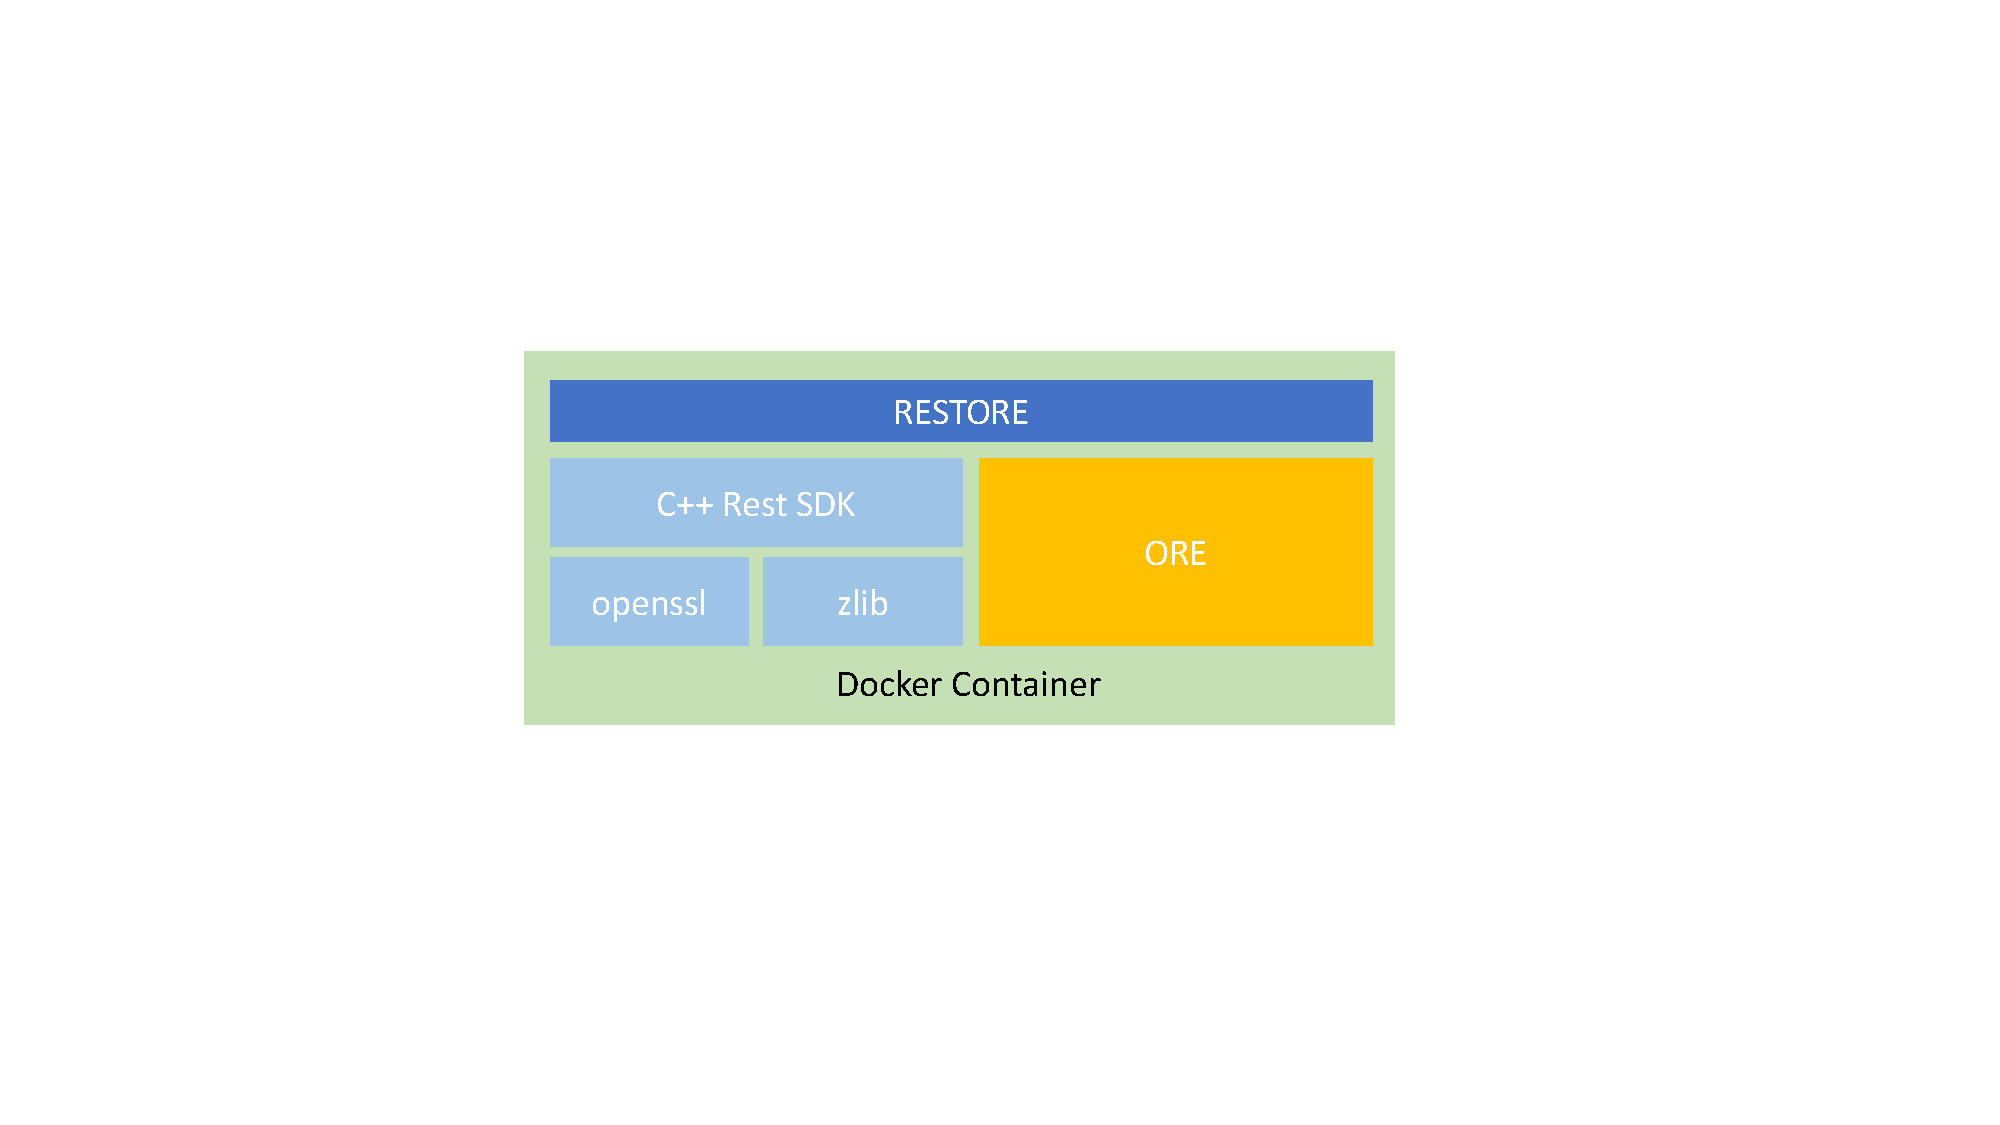
\includegraphics[scale=0.6]{data/restore.pdf}
\end{center}
\caption{RESTORE wraps ORE and uses the C++ Rest SDK to implement a RESTful API. Additional dependencies
  are openssl for authentication and zlib for compression.}
\label{fig:restore}
\end{figure}

If restore receives e.g. a pricing request it will call into other services to retrieve trade data,
market data, reference data and configurations, kick off the processing using ORE under
the hood, send the results to a data service to manage, and finally send a response to the original request. 
Figure \ref{fig:services} illustrates the communication with and between services.

\begin{figure}[h]
\begin{center}
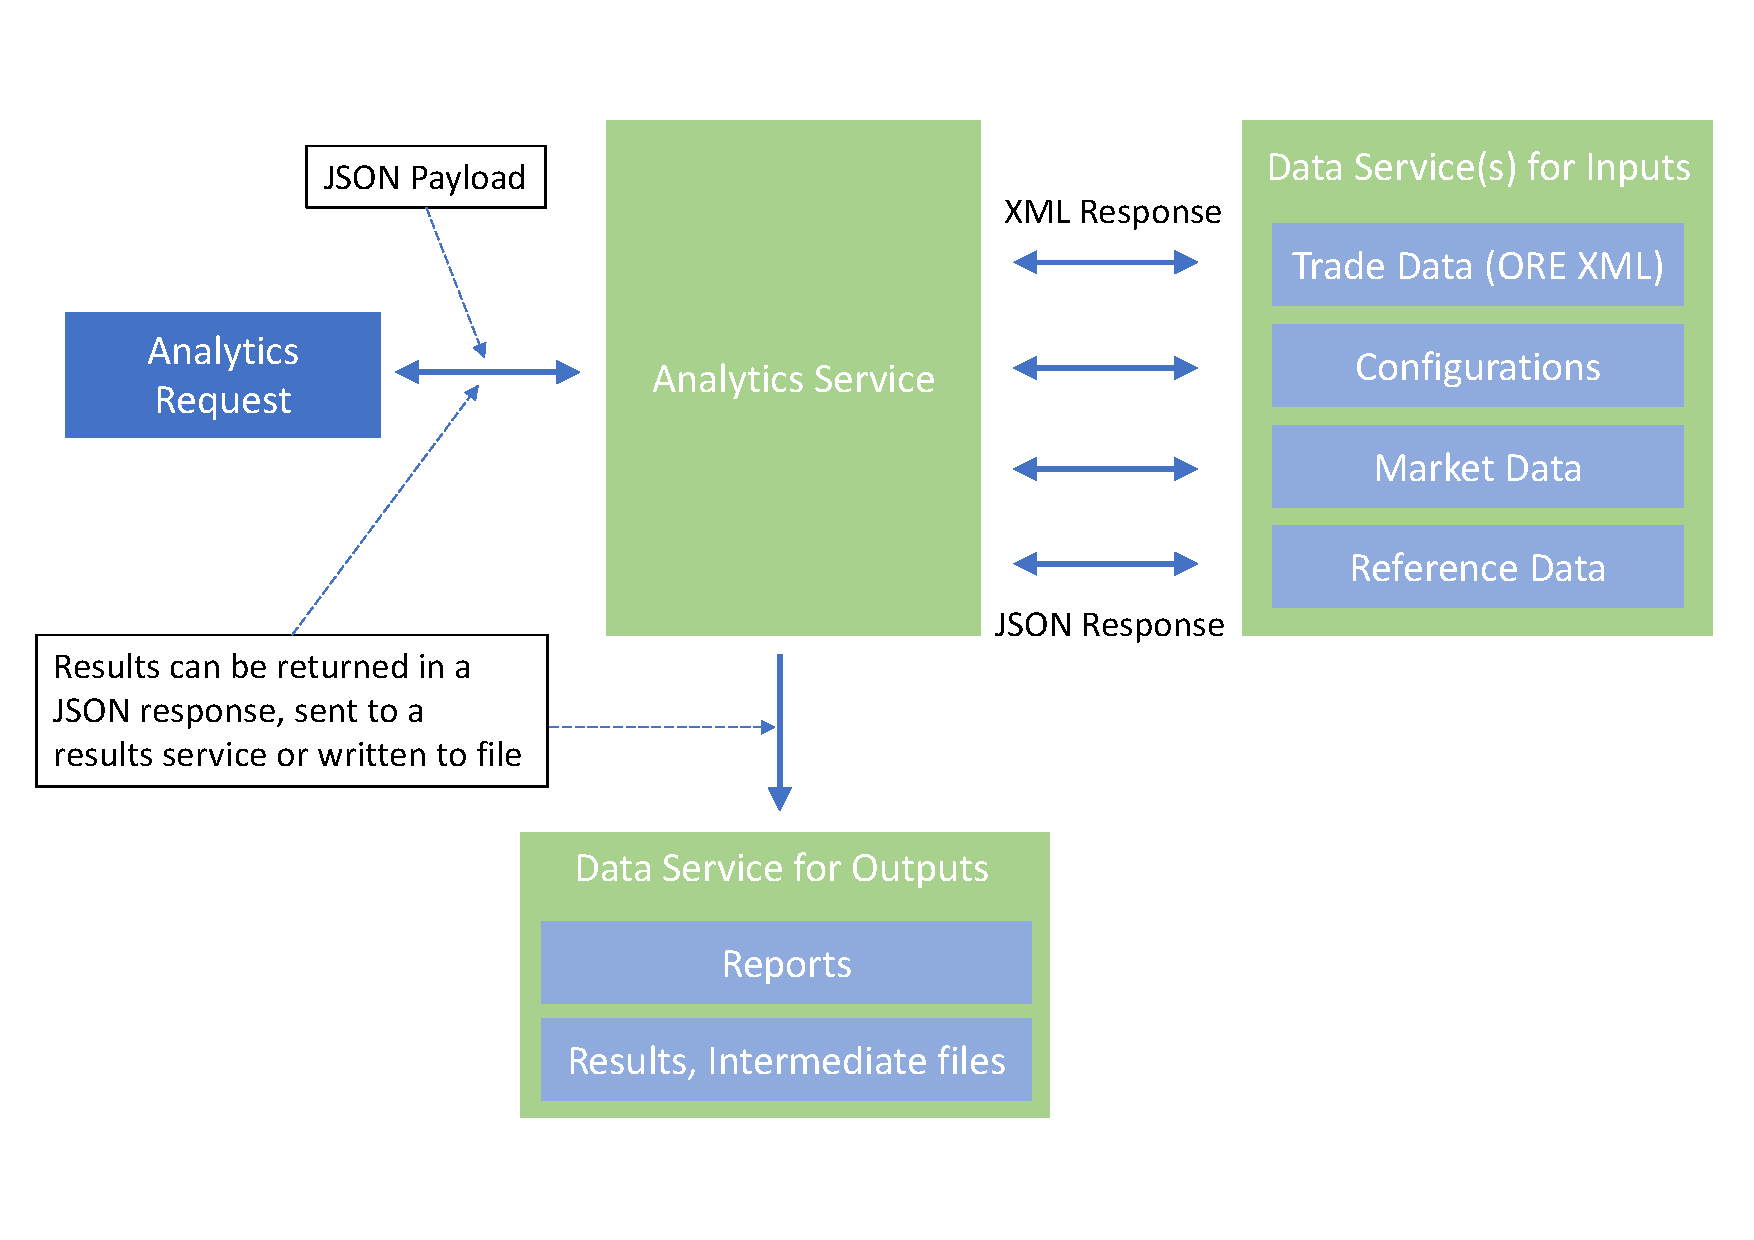
\includegraphics[scale=0.4]{data/services.pdf}
\end{center}
\caption{Request processing via the analytics service (RESTORE), data services for inputs and a
  results service.}
\label{fig:services}
\end{figure}

Before we look into restore implementation aspects, let's look at an example of how we need to structure a
typical request and how to send a request to the restore server.

Let's assume we have launched restoreserver locally with

\medskip
\centerline{\tt restoreserver ---port=5003}

to listen on port 5003.

Requests can now be sent to the server in many different ways. To test the server APIs we can use
lightweight ``clients'' such Python scripts, Postman (see https://www.postman.com), or even Emacs.
To use Python as a client, install the request package with ``pip install requests'' and send a simple
GET request to the local restoreserver to check the version of its components:

\begin{minted}[fontsize=\scriptsize]{python}
import requests
import json
url = 'http://localhost:5003/api/version'
response = requests.get(url)
print('Status:', response.status_code)
print('Response:', response.text)
print('Formatted response:', json.dumps(json.loads(response.text),indent=4))
\end{minted}

Requests can be of type GET, PUT, POST, DELETE in restore.
To ask restore to price a portfolio we need to send the following minimal POST request.

\begin{minted}[fontsize=\scriptsize]{python}
import requests
url = 'http://localhost:5003/api/pricer/default/analytics'
encoded_access_token = 'dG9rZW46dXNlcm5hbWU6cGFzc3dvcmQ='
header = { 'Authorization': 'Basic {}'.format(encoded_access_token),
           'Content-Type':'application/json'
}
body = { 'analytics': 'NPV',
         'baseCurrency': 'USD',
         'asof': 'YYYY-MM-DD',
         'portfolioUri': 'http://localhost:5000/file/portfolio.xml',
         'conventionsUri': 'http://localhost:5000/file/conventions.xml',
         'curveConfig': 'http://localhost:5000/file/curveconfig.xml',
         'scriptLibraryUri': 'http://localhost:5000/file/scriptlibrary.xml',
         'pricingEngineUri': 'http://localhost:5000/file/pricingengine.xml',
         'marketUri': 'http://localhost:5000/marketdata/market.txt/YYYY-MM-DD',
         'fixingsUri': 'https://localhost:5000/fixingdata/fixings.txt',
         'resultsPath': 'log',
         'reportUri': 'http://localhost:5000/report',
         'resultUri': 'http://localhost:5000/result',
         'outputAdditionalResults': 'true'
}
response = requests.post(url, params=body, headers=header)
print(response.text)
\end{minted}

Note:
\begin{itemize}
\item The request is sent to a different URL or {\em end point} (pricer/default/analytics).
\item We provide authorization details as part of the request header, this is typically required
\item We specify the type of content in the body of the request, via the request header 
\item We pass the ``body'' as a second argument to the request. This body of the request contains
  all information and essential URLs referencing familiar inputs that restore needs to retrieve in order to
  process the request. 
\item All URLs point to a single data service here that is running on the local host and listening on port
  5000. We have implemented a simple data service using flask for testing/demo purposes which ultimately
  reads files from the data service' input directory; one could reference several different data services
\item The report and result URIs are also pointing to the same data service, but different end points;
  these are used by the restore server to post results, in this case witten to files in the data
  service's output directory.
\item The response in this case is thin, just reports the number of successfully processed trades;
  all results are found in the data service's output directory.
\end{itemize}

RESTORE wraps additional, so far proprietary {\em ORE+} functionality that has not been
released to ORE yet, but essential for the service automation:
\begin{itemize}
\item Portfolio analyser: Determines the required market data, currencies, indexes and curves, dependent
  on portfolio and requested analytics
\item Configuration builder: Build portfolio/analytics dependent configuration on the fly, using portfolio
  analser results -- todaysmarket.xml, sensitivity.xml, simulation.xml -- so that we do not need to
  provide these in the body of the request above
\item Market data: Portfolio/analytics dependent tailoring of market data requests sent to the market data
  service
\item Reference data: Retrieve portfolio dependent reference data such as equity dividends and stock splits,
  credit index constituents and Bond static data -- so that users can simply reference a Bond via its
  security ID or a credit index by its RED code, and neither the user nor the service management team have
  to maintain such data manually
\end{itemize}

\subsubsection*{RESTORE Implemenation}

Source code components and their purpose
\begin{itemize}
\item {\bf restoreserver.cpp}: Provide main function, set global http request parameters, build
  authentication header, manage pass-through headers (?), create a server instance (RestoreHandler),
  start the server
  \begin{minted}[fontsize=\scriptsize]{c++}
    int main(int argc, char *argv[]) {
        ...
        RestoreHandler restoreHandler(address, swaggerDir, sslParameters, ptHeaders);
        try {
            // start the server
            restoreHandler.open().wait();
            ...
            restoreHandler.close().wait();
        } catch (...) {
          ...
        }
        ...
        return 0;
    }    
  \end{minted}
  Overall size about 200 lines of code
\item {\bf restorehandler.*pp}: RestoreHandler implementation; register GET, POST, PUT, DEL methods with
  the listener, only the first two linked to fully implemented functions {\tt handle\_get} and
  {\tt handle\_post}, which is sufficient for restore's purpose;
  {\tt handle\_post} eventually delegates work to {\tt handle\_analytics} and further handlers,
  all defined outside restorehandler.cpp\\
  Overall size about 500 lines of code
\item {\bf handler\_functions.*pp}: Reimplements the OREApp orchestration (eventually calling into ORE's
  analytics manager), retrieves inputs from various data service(s), manages sending results to the result
  service;\\
  Overall size about 2800 lines.
\end{itemize}
The full implementation of the restore application, used in Acadia's risk services, including all
helper classes has less than 14k lines of code, still a relatively thin ($<$ 2\%) but effective layer
on top of core ORE/QuantLib.

\begin{appendix}

%------------------------------------------------------------------------------------------------------------
\chapter{SWIG Wrapper Scope}
%------------------------------------------------------------------------------------------------------------
\label{app:swig}

ORE SWIG wrapper scope as of the 11th release, 2023.

{
\scriptsize
\begin{center}
\begin{longtable}{|l|l|}
\caption{Wrapped classes in OREAnalytics\\ \vspace{0.5cm}} \\ 
\hline
  Class & SWIG Header \\
  \hline
  Analytic & orea\_app.i \\
  AnalyticsManager & orea\_app.i \\
  InputParameters & orea\_app.i \\
  MarketDataInMemoryLoader & orea\_app.i \\
  OREApp & orea\_app.i \\
  Parameters & orea\_app.i \\
  AggregationScenarioData & orea\_cube.i \\
  NPVCube & orea\_cube.i \\
  \hline
\end{longtable}
\end{center}
}

{
\scriptsize
\begin{longtable}{|l|l|}
\caption{Wrapped classes in OREData \\ \vspace{0.5cm}} \\
\hline
Class & SWIG Header \\
\hline
CalendarAdjustmentConfig & ored\_calendarAdjustmentConfig.i \\
AverageOisConvention & ored\_conventions.i \\
BMABasisSwapConvention & ored\_conventions.i \\
CdsConvention & ored\_conventions.i \\
Convention & ored\_conventions.i \\
Conventions & ored\_conventions.i \\
CrossCcyBasisSwapConvention & ored\_conventions.i \\
CrossCcyFixFloatSwapConvention & ored\_conventions.i \\
DepositConvention & ored\_conventions.i \\
FXConvention & ored\_conventions.i \\
FraConvention & ored\_conventions.i \\
FutureConvention & ored\_conventions.i \\
IRSwapConvention & ored\_conventions.i \\
InflationSwapConvention & ored\_conventions.i \\
OisConvention & ored\_conventions.i \\
SecuritySpreadConvention & ored\_conventions.i \\
SwapIndexConvention & ored\_conventions.i \\
TenorBasisSwapConvention & ored\_conventions.i \\
TenorBasisTwoSwapConvention & ored\_conventions.i \\
ZeroRateConvention & ored\_conventions.i \\
BaseCorrelationCurveSpec & ored\_curvespec.i \\
CDSVolatilityCurveSpec & ored\_curvespec.i \\
CapFloorVolatilityCurveSpec & ored\_curvespec.i \\
CommodityCurveSpec & ored\_curvespec.i \\
CommodityVolatilityCurveSpec & ored\_curvespec.i \\
CorrelationCurveSpec & ored\_curvespec.i \\
CurveSpec & ored\_curvespec.i \\
DefaultCurveSpec & ored\_curvespec.i \\
EquityCurveSpec & ored\_curvespec.i \\
EquityVolatilityCurveSpec & ored\_curvespec.i \\
FXSpotSpec & ored\_curvespec.i \\
FXVolatilityCurveSpec & ored\_curvespec.i \\
InflationCapFloorVolatilityCurveSpec & ored\_curvespec.i \\
InflationCurveSpec & ored\_curvespec.i \\
SecuritySpec & ored\_curvespec.i \\
SwaptionVolatilityCurveSpec & ored\_curvespec.i \\
YieldCurveSpec & ored\_curvespec.i \\
YieldVolatilityCurveSpec & ored\_curvespec.i \\
CSVLoader & ored\_loader.i \\
InMemoryLoader & ored\_loader.i \\
Loader & ored\_loader.i \\
BufferLogger & ored\_log.i \\
FileLogger & ored\_log.i \\
Log & ored\_log.i \\
Logger & ored\_log.i \\
MarketImpl & ored\_market.i \\
TodaysMarket & ored\_market.i \\
BMASwapQuote & ored\_marketdatum.i \\
BaseCorrelationQuote & ored\_marketdatum.i \\
BasisSwapQuote & ored\_marketdatum.i \\
BondOptionQuote & ored\_marketdatum.i \\
BondOptionShiftQuote & ored\_marketdatum.i \\
BondPriceQuote & ored\_marketdatum.i \\
CPRQuote & ored\_marketdatum.i \\
CapFloorQuote & ored\_marketdatum.i \\
CapFloorShiftQuote & ored\_marketdatum.i \\
CdsQuote & ored\_marketdatum.i \\
CommodityForwardQuote & ored\_marketdatum.i \\
CommodityOptionQuote & ored\_marketdatum.i \\
CommoditySpotQuote & ored\_marketdatum.i \\
CorrelationQuote & ored\_marketdatum.i \\
CrossCcyBasisSwapQuote & ored\_marketdatum.i \\
CrossCcyFixFloatSwapQuote & ored\_marketdatum.i \\
DiscountQuote & ored\_marketdatum.i \\
EquityDividendYieldQuote & ored\_marketdatum.i \\
EquityForwardQuote & ored\_marketdatum.i \\
EquityOptionQuote & ored\_marketdatum.i \\
EquitySpotQuote & ored\_marketdatum.i \\
FRAQuote & ored\_marketdatum.i \\
FXForwardQuote & ored\_marketdatum.i \\
FXOptionQuote & ored\_marketdatum.i \\
FXSpotQuote & ored\_marketdatum.i \\
HazardRateQuote & ored\_marketdatum.i \\
ImmFraQuote & ored\_marketdatum.i \\
IndexCDSOptionQuote & ored\_marketdatum.i \\
InflationCapFloorQuote & ored\_marketdatum.i \\
MMFutureQuote & ored\_marketdatum.i \\
MarketDatum & ored\_marketdatum.i \\
MoneyMarketQuote & ored\_marketdatum.i \\
OIFutureQuote & ored\_marketdatum.i \\
RecoveryRateQuote & ored\_marketdatum.i \\
SeasonalityQuote & ored\_marketdatum.i \\
SecuritySpreadQuote & ored\_marketdatum.i \\
SwapQuote & ored\_marketdatum.i \\
SwaptionQuote & ored\_marketdatum.i \\
SwaptionShiftQuote & ored\_marketdatum.i \\
YoYInflationSwapQuote & ored\_marketdatum.i \\
YyInflationCapFloorQuote & ored\_marketdatum.i \\
ZcInflationCapFloorQuote & ored\_marketdatum.i \\
ZcInflationSwapQuote & ored\_marketdatum.i \\
ZeroQuote & ored\_marketdatum.i \\
EngineBuilder & ored\_portfolio.i \\
EngineData & ored\_portfolio.i \\
EngineFactory & ored\_portfolio.i \\
Envelope & ored\_portfolio.i \\
InstrumentWrapper & ored\_portfolio.i \\
LegBuilder & ored\_portfolio.i \\
Portfolio & ored\_portfolio.i \\
Trade & ored\_portfolio.i \\
TradeFactory & ored\_portfolio.i \\
PlainInMemoryReport & ored\_reports.i \\
GenericYieldVolCurve & ored\_volcurves.i \\
LocalVolModelBuilder & ored\_volcurves.i \\
SwaptionVolCurve & ored\_volcurves.i \\
\hline
\end{longtable}
%\end{center}
}

{
\scriptsize
\begin{longtable}{|l|l|}
\caption{Wrapped classes in QuantExt \\ \vspace{0.5cm}} \\
\hline
Class & SWIG Header \\
\hline
AverageOIS & qle\_averageois.i \\
AverageONIndexedCouponPricer & qle\_averageois.i \\
AverageOISRateHelper & qle\_averageoisratehelper.i \\
Belgium & qle\_calendars.i \\
CME & qle\_calendars.i \\
Colombia & qle\_calendars.i \\
Cyprus & qle\_calendars.i \\
Greece & qle\_calendars.i \\
ICE & qle\_calendars.i \\
Ireland & qle\_calendars.i \\
IslamicWeekendsOnly & qle\_calendars.i \\
LargeJointCalendar & qle\_calendars.i \\
Luxembourg & qle\_calendars.i \\
Malaysia & qle\_calendars.i \\
Netherlands & qle\_calendars.i \\
Peru & qle\_calendars.i \\
Philippines & qle\_calendars.i \\
RussiaModified & qle\_calendars.i \\
Spain & qle\_calendars.i \\
Wmr & qle\_calendars.i \\
FXLinkedCashFlow & qle\_cashflows.i \\
FloatingRateFXLinkedNotionalCoupon & qle\_cashflows.i \\
CrossCcySwap & qle\_ccyswap.i \\
CrossCcySwapEngine & qle\_ccyswap.i \\
AverageONIndexedCoupon & qle\_coupons.i \\
AverageONLeg & qle\_coupons.i \\
CapFlooredAverageONIndexedCouponPricer & qle\_coupons.i \\
CappedFlooredAverageONIndexedCoupon & qle\_coupons.i \\
QLEBlackCdsOptionEngine & qle\_creditdefaultswap.i \\
QLECdsOption & qle\_creditdefaultswap.i \\
CrossCcyFixFloatSwap & qle\_crossccyfixfloatswap.i \\
DiscountingEquityForwardEngine & qle\_equityforward.i \\
EquityForward & qle\_equityforward.i \\
BEHICP & qle\_indexes.i \\
BMAIndex & qle\_indexes.i \\
BMAIndexWrapper & qle\_indexes.i \\
BondFuturesIndex & qle\_indexes.i \\
BondIndex & qle\_indexes.i \\
CommodityFuturesIndex & qle\_indexes.i \\
CommodityIndex & qle\_indexes.i \\
CommoditySpotIndex & qle\_indexes.i \\
ConstantMaturityBondIndex & qle\_indexes.i \\
EquityIndex2 & qle\_indexes.i \\
FxIndex & qle\_indexes.i \\
Name & qle\_indexes.i \\
CommodityForward & qle\_instruments.i \\
CrossCcyBasisMtMResetSwap & qle\_instruments.i \\
CrossCcyBasisSwap & qle\_instruments.i \\
Deposit & qle\_instruments.i \\
DepositEngine & qle\_instruments.i \\
DiscountingCommodityForwardEngine & qle\_instruments.i \\
DiscountingFxForwardEngine & qle\_instruments.i \\
DiscountingSwapEngineMultiCurve & qle\_instruments.i \\
FxForward & qle\_instruments.i \\
GeneralisedReplicatingVarianceSwapEngine & qle\_instruments.i \\
OvernightIndexedBasisSwap & qle\_instruments.i \\
Payment & qle\_instruments.i \\
PaymentDiscountingEngine & qle\_instruments.i \\
VarianceSwap2 & qle\_instruments.i \\
OvernightIndexedCrossCcyBasisSwap & qle\_oiccbasisswap.i \\
OvernightIndexedCrossCcyBasisSwapEngine & qle\_oiccbasisswap.i \\
BasisTwoSwapHelper & qle\_ratehelpers.i \\
CrossCcyBasisMtMResetSwapHelper & qle\_ratehelpers.i \\
CrossCcyBasisSwapHelper & qle\_ratehelpers.i \\
CrossCcyFixFloatSwapHelper & qle\_ratehelpers.i \\
ImmFraRateHelper & qle\_ratehelpers.i \\
OIBSHelper & qle\_ratehelpers.i \\
OICCBSHelper & qle\_ratehelpers.i \\
SubPeriodsSwapHelper & qle\_ratehelpers.i \\
TenorBasisSwapHelper & qle\_ratehelpers.i \\
SubPeriodsCoupon1 & qle\_tenorbasisswap.i \\
SubPeriodsSwap & qle\_tenorbasisswap.i \\
TenorBasisSwap & qle\_tenorbasisswap.i \\
BlackVarianceSurfaceMoneynessForward & qle\_termstructures.i \\
BlackVarianceSurfaceMoneynessSpot & qle\_termstructures.i \\
BlackVolatilityWithATM & qle\_termstructures.i \\
CreditCurve & qle\_termstructures.i \\
CreditVolCurve & qle\_termstructures.i \\
CreditVolCurveWrapper & qle\_termstructures.i \\
FxBlackVannaVolgaVolatilitySurface & qle\_termstructures.i \\
Name & qle\_termstructures.i \\
PriceTermStructure & qle\_termstructures.i \\
QLESwaptionVolCube2 & qle\_termstructures.i \\
SwapConventions & qle\_termstructures.i \\
SwaptionVolCubeWithATM & qle\_termstructures.i \\
SwaptionVolatilityConstantSpread & qle\_termstructures.i \\
SwaptionVolatilityConverter & qle\_termstructures.i \\
\hline
\end{longtable}
}

\end{appendix}

%-------------------------------------------------------------------------------
\begin{thebibliography}{*}

\bibitem{ORE} Open Source Risk Engine, A Free Open-ource Platform for Risk Analytics and XVA, http://opensourcerisk.org, https://github.com/opensourcerisk

\bibitem{QuantLib} QuantLib, A Free Open-Source Library for Quantitative Finance, http://www.quantlib.org

\bibitem{ballabio_book} L.~Ballabio, ``Implementing QuantLib - Quantitative Finance in C++: an inside look at the architecture of the QuantLib library'', \url{https://leanpub.com/implementingquantlib}

\bibitem{ballabio_blog}  L.~Ballabio, ``Implementing QuantLib'' blog posts on \url{https://www.implementingquantlib.com}
\bibitem{autodiff}
Community portal to automatic differentiation (AD),
\url{http://www.autodiff.org}

\bibitem{griewank_2000}
A.~Griewank.
\newblock {\em {Evaluating derivatives: principles and techniques of
  algorithmic differentiation}}.
\newblock Society for Industrial and Applied Mathematics, 2000.

\bibitem{giles_2006} M.~Giles and P.~Glasserman,
Smoking adjoints: fast Monte Carlo Greeks, {\em RISK}, January 2006.

\bibitem{leclerc_2009}
M.~Leclerc, Q.~Liang, and I.~Schneider.
\newblock {Fast Monte Carlo Bermudan Greeks}.
\newblock {\em RISK}, July 2009.

\bibitem{joshi_2010}
M.~Joshi and C.~Yang.
\newblock {Fast Gamma computations for CDO tranches}.
\newblock {\em http://ssrn.com/paper=1689348}, 2010.

\bibitem{capriotti_2010}
L.~Capriotti and M.B. Giles.
\newblock {Fast correlation Greeks by adjoint algorithmic differentiation}.
\newblock {\em RISK}, March, 2010.

\bibitem{capriotti_2011}
L.~Capriotti.
\newblock {Fast Greeks by algorithmic differentiation}.
\newblock {\em Journal of Computational Finance}, 4:3--35, 2011.

\bibitem{capriotti_2011b}
L.~Capriotti and M.B. Giles.
\newblock {Algorithmic differentiation: Adjoint Greeks made easy}.
\newblock {\em http://ssrn.com/paper=1801522}, 2011.

\bibitem{capriotti_2011c}
L.~Capriotti, S.~Lee, and M.~Peacock.
\newblock {Real time counterparty credit risk management in Monte Carlo}.
\newblock {\em http://ssrn.com/paper=1824864}, 2011.

\bibitem{sherif_2015}
N.~Sherif.
\newblock {AAD vs GPU: banks turn to maths trick as chips lose appeal}.
\newblock {\em RISK}, January 2015.

\bibitem{fries_2017_1}
  C.~Fries, Stochastic Automatic Differentiation: Automatic Differentiation for Monte-Carlo Simulations, 2017, \url{https://ssrn.com/abstract=2995695}

\bibitem{fries_2017_2}
  C.~Fries, Automatic Backward Differentiation for American Monte-Carlo Algorithms - ADD for Conditional Expectations and Indicator Functions, 2017, \url{https://ssrn.com/abstract=3000822}

\bibitem{fries_2017_3}
  C.~Fries, Fast Stochastic Forward Sensitivities in Monte-Carlo Simulations Using Stochastic Automatic Differentiation (with Applications to Initial Margin Valuation Adjustments (MVA)), 2017, \url{https://ssrn.com/abstract=3018165}

\bibitem{savine_cg_1} A:~Savine,
  Computation Graphs for AAD and Machine Learning Part I: \\
  Introduction to Computation Graphs and Automatic Differentiation, 2019,\\
  \url{https://www.researchgate.net/publication/337201082_Computation_Graphs_for_AAD_and_Machine_Learning_Part_I_Introduction_to_Computation_Graphs_and_Automatic_Differentiation}

\bibitem{savine_cg_2} A:~Savine,
  Computation Graphs for AAD and Machine Learning Part II: \\
  Adjoint Differentiation and AAD, 2020\\
  \url{https://www.researchgate.net/publication/338662793_Computation_Graphs_for_AAD_and_Machine_Learning_Part_II_Adjoint_Differentiation_and_AAD}

\bibitem{savine_cg_3} A:~Savine,
  Computation Graphs for AAD and Machine Learning Part III: \\
  Application to Derivatives Risk Sensitivities, 2020, \\
  \url{https://www.researchgate.net/publication/340126636_Computation_Graphs_for_AAD_and_Machine_Learning_Part_III_Application_to_Derivatives_Risk_Sensitivities}

\bibitem{savine_book_1} A:~Savine and L.~Andersen
  Modern Computational Finance: AAD and Parallel Simulations,
  Wiley, 2018

\bibitem{savine_book_2} A:~Savine and J.~Andreasen,
  Modern Computational Finance: Scripting for Derivatives and xVA
  Wiley, 2021

\bibitem{swig} Simplified Wrapper Interface Generator, \url{https://www.swig.org}
  
\end{thebibliography}


\end{document}
